%
% File: chap01.tex
% Author: Ran Itay
% Description: Introduction chapter.
%
\let\textcircled=\pgftextcircled
\chapter{Introduction}
\label{chap:intro}

\initial{T}he most accredited theoretical framework for the cosmology of our universe, based on numerous cosmological and astronomical observations, is the "$\Lambda$-Cold Dark Matter" model (\cdm). It suggests that only a small fraction ($\sim 5\%$) of the energy density in the universe is in the form of baryonic matter, the rest  $\sim 95\%$ is lurking in the dark~\cite{WMAP:9years, Planck}. The "Dark-sector" consist of \textit{Dark Energy}($\sim 69\%$) and a non-baryonic matter ($\sim 26\%$), \textit{Dark Matter} (DM).

In the 1930s the Swiss astronomer Fritz Zwicky observed that the mass of the cluster inferred by gravitational observation is much larger than the one inferred by the visible luminous light matter. He then deduced the existence of a new type of unseen matter which does not interact with electromagnetic radiation, naming this matter \textit{"dunkle materie"}, \textit{Dark Matter}~\cite{Zwicky:1937zza}. Since then much evidence has been accumulated, suggesting that DM is present at galactic as well as cosmological scales.

In the past decade many experiments joined the race towards DM detection, and the field has progressed dramatically. These experiments can be divided
roughly into three groups, underground direct detection experiments such as XENON~\cite{xe100_run_combination,Xenon1TResults}, LUX~\cite{LUXnew}, PANDAX~\cite{PANDAX}, CDMS~\cite{CDMSlite}, DAMA/LIBRE~\cite{DAMA} and others , indirect detection in space (FERMI~\cite{FermiLAT:2011ab}, AMS~\cite{AMS}) and on earth (IceCube~\cite{IceCube}), and production experiments in accelerators such as ATLAS~\cite{AtlasDM} and CMS~\cite{CmsDM} at the Large Hadron Collider.
\section{Evidence for the Existence Of Dark Matter}
\label{sec:Evidence}
An extensive amount of observations pointing to the presence of DM at the  single--galaxy, inter-galactic and cosmological scales, are present. In this section a brief summary of these observation is presented. 

\subsection{Virial Theorem}
\label{subsec:virial}
The virial theorem relates the average potential energy density $\left\langle V_p \right\rangle$ of a stationary gravitationally bound system to its mean kinetic energy density $\left\langle T_k \right\rangle $, namely:
\begin{equation}
\left\langle T_k \right\rangle  =-\frac{1}{2}\left\langle V_p \right\rangle.
\end{equation}


In the 1930s Zwicky made the puzzling observation that the velocity dispersion of individual nebulae in the large Coma galaxy cluster contradicts the expectation of the virial theorem, if estimating the total mass solely from the visible matter content~\cite{Zwicky:1937zza}. Additional mass in the form of DM needs to be added to explain the observations. Although Zwicky did not take into account the mass of the hot plasma in the cluster, adding it reduces the discrepancies but doesn't solve it. 

The hot plasma bounded by the gravitational potential of the cluster emits bremsstrahlung X-rays. The x-ray emission is proportional to the plasma density squared. This can be used to estimate the the total mass and mass profile of clusters assuming the cluster is virialized. This type of observations suggest that DM rather than baryonic matter dominates the dynamics of clusters~\cite{Lewis:2002mfa}.

 


\subsection{Galactic Rotation Curves}
\label{subsec:RotCurve}
The orbital velocity as a function of radius (rotation curve) can be obtained from the measurement of the redshifts of the 1420\,MHz hydrogen transition~\cite{Begeman:1991iy} as well as of spectral lines from stars. The hydrogen cloud extends beyond the galactic disk, allowing the measurement of orbital velocities further out. By measuring the rotation curve of galaxies it is possible to compute their mass profile ($\textrm{M}(r)$).

In 1970 Vera Rubin found a disagreement in the mass profile calculated by the rotation curves and the one expected from luminouse mattter in NGC4605 spiral galaxy~\cite{Rubin:1980zd}. This disagreement can be solved, assuming additional non-visible mass enhancing the gravitational forces.

Formally, assuming Newtonian dynamics
\begin{equation}
\label{v_r}
v(r) = \sqrt{\frac{\mathrm{G}\cdot \mathrm{M}(r)}{r}},
\end{equation} 
where
\begin{equation}
\label{M_r}
\mathrm{M}(r) =  \int_o^r 4\pi \rho(r)r^2dr.
\end{equation}
The majority of a galaxy's luminous mass is situated at the close vicinity of its center  ; therefore if no other mass exist, at large radii one would expect $v(r) \sim r^{-1/2}$. In contradiction the measurements done by Rubin and in many more experiments indicate $v(r) \sim \mathrm{const}$, see Fig.~\ref{fig:RotationCurve}. Adding DM with density profile $\rho(r) \sim r^{-2}$ explains this observations.

 \begin{figure}[]
	\centering
	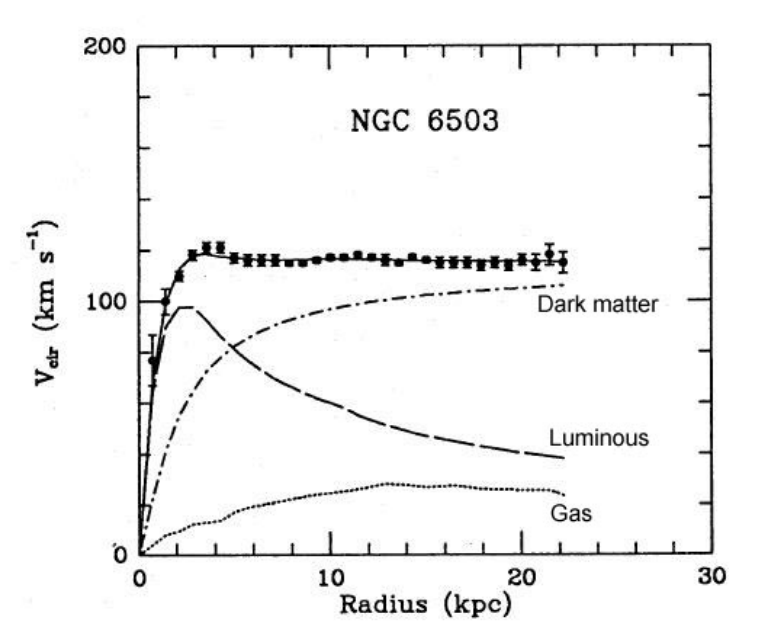
\includegraphics[width=0.8\textwidth]{figs/rotationCurve6503.png}
	\mycaption[Rotation curve of NGC 6503.]{Measured Rotation curve (solid line) of NGC 6503 galaxy. In dashed, luminous component only. In dotted, the gas component, and expected DM halo in dotted-dashed. Image taken from ~\cite{Begeman:1991iy}.}
	\label{fig:RotationCurve}
\end{figure}  

\subsection{Gravitational Lensing}
  
One of the predictions of general relativity is that trajectory of light in space is determined by the space-time metric, which is determined by the mass distribution. Due to this effect, when a large gravitational potential is located in the line of sight between an observer and a far galaxy, the light from the galaxy is distorted. This phenomena is called Gravitational Lensing~\cite{Bertone:2010zza}. By analyzing the lensed image, the mass profile of the "lens" can be characterized.

\textit{Strong Lensing} is when the gravitational field of the "lens" is so strong it produces multiple images forming an Einstien's cross, as well as Einstein's rings~\cite{Einstein:1956zz}. In Fig.~\ref{subfig:abell1689} is a picture of the largest lensing galaxy cluster observed, Abell 1689. In Fig.~\ref{subfig:QSO} is the a lensed, multiple image picture of the quasar QSO-2237. 

\begin{figure}
   \centering
    \begin{minipage}[c]{0.38\textwidth}
    \centering
    \subbottom[]{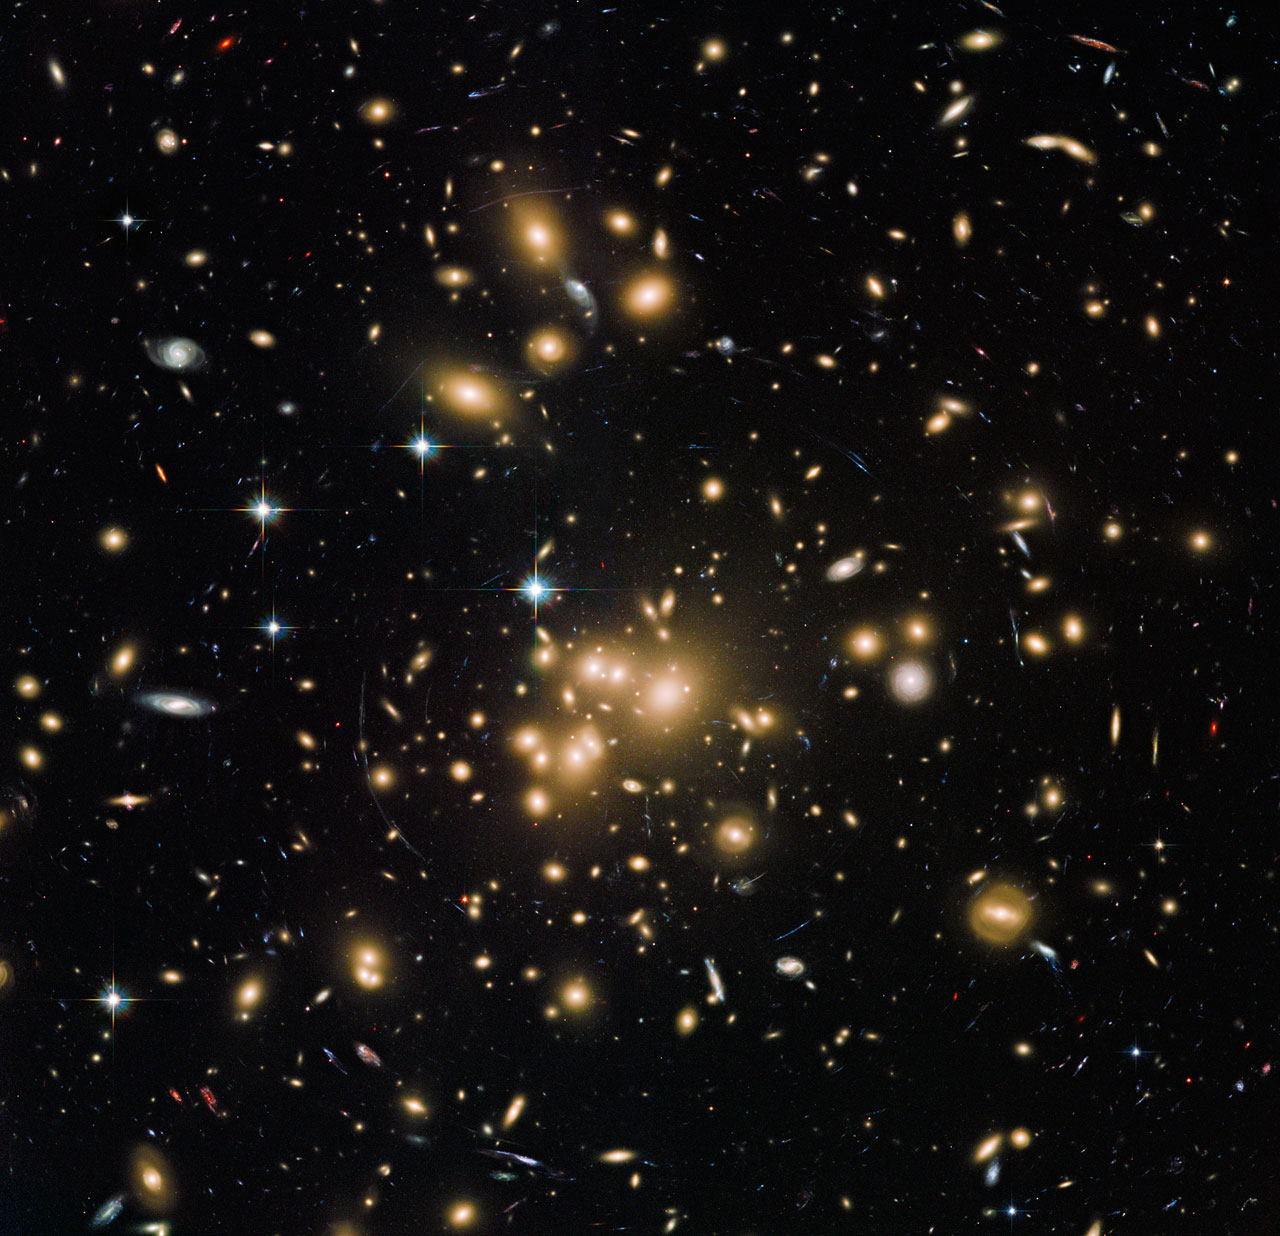
\includegraphics[width=\textwidth]{figs/hubel1689.jpg}
%        \caption{The cryostat and the collimator shining just some of the FV }
        \label{subfig:abell1689}}
    \end{minipage}
    \begin{minipage}[c]{0.4\textheight}%0.49\textwidth , 0.9\textheight}
	\centering    
        \subbottom[]{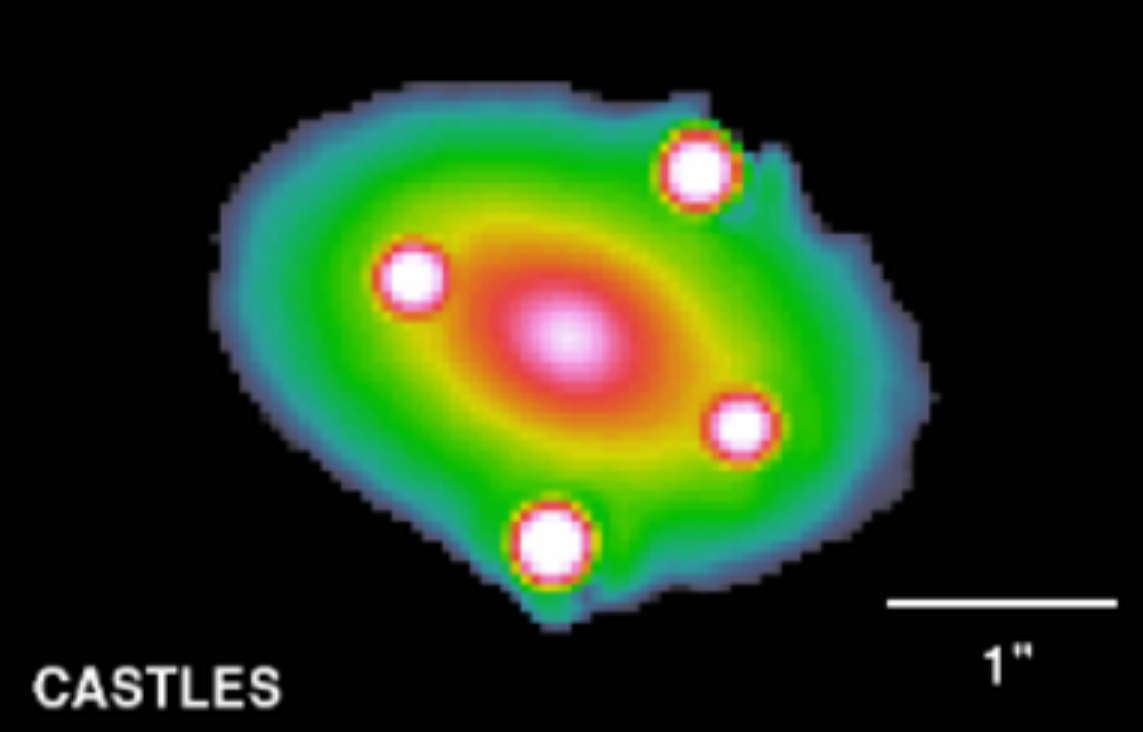
\includegraphics[width=\textwidth]{figs/QSO.png}
%        \caption{a CAD design of the collimator with the conical hole.}
        \label{subfig:QSO}}
    \end{minipage} 
    \mycaption[Strong lensing]{ (a) Hubble Space Telescope Advanced Camera for Surveys image of the lensing cluster Abell 1689. Image credit: ESA/Hubble. (b) QSO-2237 quaser lensed image, creating both einstein's arcs and cross. Image credit: CASTLES \label{fig:StrongLens}}
\end{figure}

Two important features are concuded when analyzing the mass profile of the "lens": 1) DM and ordinary matter are not misaligned~\cite{Ferreras:2007na}. 2) The mass profile follows $\rho(r)\propto r^{-2}$ dispersion ratio~\cite{Gavazzi:2007vw}. 

\textit{Weak Lensing} is when the light coming from the source is only weakly distorted by the gravitational lens. In this case it is impossible to detect an individual lensed source; however, multiple background sources align symmetrically around the lens, allowing the detection of the lens mass~\cite{Kaiser:1992ps}.

The most famous weak lensing evidence for DM comes from the "Bullet Cluster", a lensed image of a collision of two galaxies, 1E0657-56 and MACS J0025.4-1222~\cite{Clowe:2006eq}. In this observation (see Fig.~\ref{fig:Bullet}), it is clear that the mass distribution of the luminous and non-luminous matters are spatially displaced. While the luminous matter seems to experienced a violent collision, the non-lominous matter seems to be unaffected. The collisionless behaviour of the DM puts strong constrains on its self inteaction~\cite{Randall:2007ph}. 

 \begin{figure}[]
	\centering
	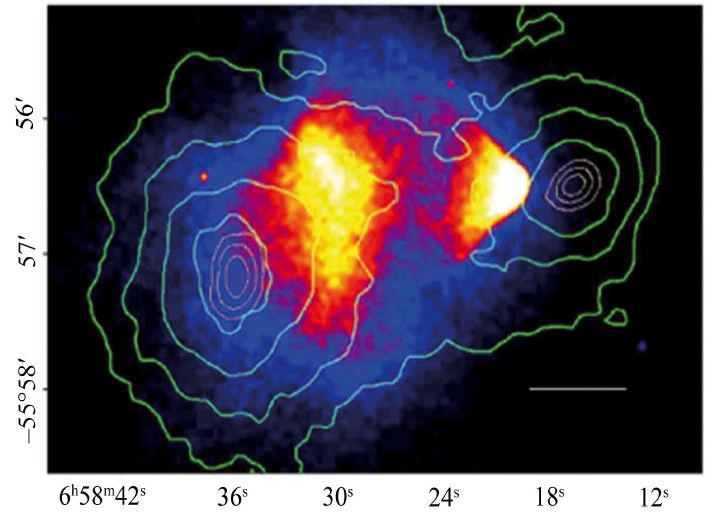
\includegraphics[width=0.8\textwidth]{figs/bulletCluster.jpg}
	\mycaption[Bullet Cluster]{Contours of spatial distribution of mass, from gravitational lensing overplotted over Chandra x-ray data that traces hot plasma in a galaxy. It can be seen that most of the matter resides in a location different from the plasma, which underwent frictional interactions during the merger and slowed down.}
	\label{fig:Bullet}
\end{figure}  



\subsection{Cosmic Microwave Background}
The most precise constraint of the abundance of dark matter in the Universe and a landmark test on the \cdm\ model comes from the measurements of the cosmic microwave background (CMB). The CMB is a reminisce thermal electromagnetic radiation field from the early Universe. 

At the early stages of the Universe, it was hot, dense, and filled with plasma. Then after expanding enough the temperature dropped, and electrons and protons  recombined creating hydrogen atoms. At that stage (reffed as "recombination time"), as the density of free electrons dropped, the thermal radiation could travel freely, without being scattered. These photons propagate through the Universe ever since.       

The CMB follows with extreme precision the spectrum of a black body with temperature of 2.726\,K. It is also known to be very isotropic and temperature  anisotropy is at the scale of $10\mu$K. These temperature fluctuations, considered Gaussian~\cite{WMAP:9years}, are usually expanded using spherical harmonics,
\begin{equation}
\frac{\delta T }{T}(\theta,\phi) = \sum_{l=2}^{\infty}\sum_{m=-l}^{m=l}a_{lm}Y_{lm}(\theta,\phi). 
\end{equation} 

The variance of the coefficient $a_{lm}$ denoted as $c_l$ is defined:
\begin{equation}
c_l \equiv \left< a_{lm} \right> = \frac{1}{2l+1}\sum_{m=-1}^{m=l}a_{lm}^2
\end{equation}

All DM relevance information from CMB can be extracted from the power spectrum of $c_l$ as a function of the multipole $l$. The shape of the power spectrum follows the oscillations of the plasma in the early Universe. In general, the flatness of the Universe can be extracted from the position of the first peak. The ratio between the baryonic and non-baryonic matter is extracted from the ratio between the first two peaks.   

More specifically, there are many parameters which affect the CMB spectrum, amongst them are the DM density ($\Omega_{DM}$), the baryonic matter density ($\Omega_{b}$) and the Hubble constant ($h$). Assuming a cosmological model with fixed number of parameters the best fit to the spectrum determines the values of the parameters. The most updated measurment of the CMB spectrum seen in Fig~\ref{fig:CMB} constraine the values of the above mentioned parameters~\cite{Planck} to:
\begin{equation}
\Omega_{DM}h^2 = 0.1197 \pm 0.0022 \qquad \Omega_{b}h^2 = 0.00222 \pm 0.00023 \qquad h=0.67\;[100\, \mathrm{km/s/Mpc}] 
\end{equation}

\begin{figure}[]
	\centering
	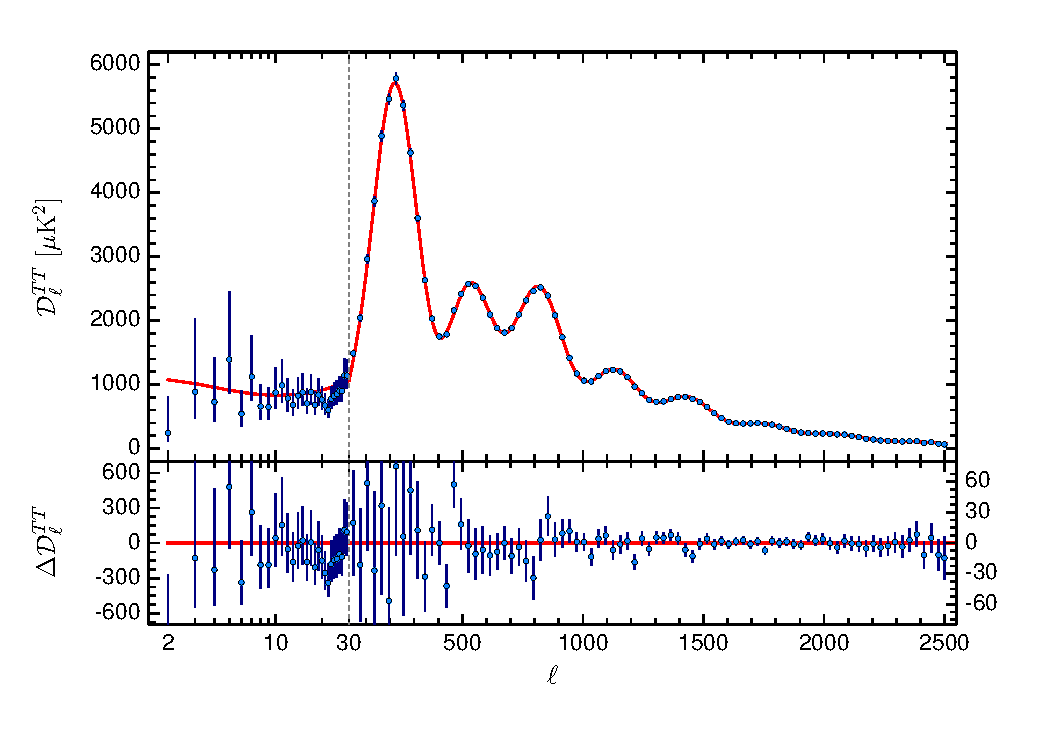
\includegraphics[width=\textwidth]{figs/planck.pdf}
	\mycaption[Plank 2015 CMB power spectrum] {The Planck 2015 temperature power spectrum the solid line is the best fit for the \cdm\ model, the error bars show $\pm \sigma$ uncertainties}
	\label{fig:CMB}
\end{figure}  
  
\subsection{Big Bang Nucleosynthesis}
\label{subsec:BBN}
Big Bang Nucleosynthesis (BBN) is a theory describing the production of the lightest nuclei via a dynamic interplay amongst the four fundamental forces during the first seconds of the Universe~\cite{Jedamzik:2009uy}. The BBN process started when the Universe expanded and became cold enough for electrons and protons to recombine, creating light elements such as Helium, Deuterium, and Lithium, it lasted $\sim20$\,min.

The abundance of the lightest nuclei created in the BBN era can be parametrized by the baryonic density $\Omega_b$ only. This can be done as DM doesn't affect      the expansion rate of the Universe, because the Universe is radiation dominant. The inferred value of $\Omega_b$ which gives the correct abundance, coincide with the one measured by CMB, supporting the existence of non-baryonic matter constituting a large fraction of the matter in the Universe. 
\section{Particle Candidates and Other Solutions to the Dark Matter Problem }
As discussed in previous section there is a large number of convincing evidences for supporting the existence of DM in the Universe, of which its nature is yet unknown. In this section is a short discussion of possible candidates for DM particles, as well as an alternative solution involving the modification of Newton's laws.

\subsection{Axions}

Axions are neutral pseudoscalars initially introduced by Peccei and Quinn in 1977 to solve the "strong CP problem"~\cite{Peccei:1977hh}. The Standard model of particles (SM) contains a CP violating proportional to the parameter $\bar{\theta} = \theta_{weak}+ arg(det(M))$. From measurements  of the electrical dipole moment of the neutron the $\bar{\theta}$ parameter is constrained to be smaller than $10^{-10}$~\cite{Pospelov:2005pr,Baker:2006ts}. The question why the $\bar{\theta}$ parameter is so small is known as the strong CP problem. An elegant solution to this problem is introducing an additional global $U(1)$ symmetry, spontaneously broken producing a Goldstone boson known as the axion. 

Many theoretical and experimental efforts were invested in axion search. The original proposed Peccei-Quinn axion with symmetry breaking scale in the order of the weak scale (246\,GeV) is ruled out; however, axion and axion like particles (ALPs) are still allowed~\cite{Kim:1979if,Akerib:2017uem} 

\subsection{Primordial Black Holes}
primordial black hole (PBH) are a postulated type of black holes formed at the era before BBN, thus they are not subject to the baryon to photon ration, which gives the baryon density. They were first introduced by Stephen Hawking~\cite{PBH} at 1971, and they can theoretically account for fraction of the DM density~\cite{Carr:2016drx}. 

Limits on the mass of PBH can be placed from the lack
of Hawking-radiated gamma-rays~\cite{MacGibbon:1987my}, combined with null results from microlensing surveys, and constraints based on the CMB~\cite{Ricotti:2007au}. The current allowed mass range of of DM in the form of PBH is ($10^{14}$--$10^{23}$)\,kg.

\subsection{Modified Newtonian Dynamics}
\label{subsec:MOND}

Although the cold dark matter paradigm solves the problems arising from several observations that are mentioned above, there are other paradigms that answer this puzzling observations. The most reasonable is Modified Newtonian Dynamics (MOND)~\cite{Milgrom:1983ca} suggested by Mordechai Milgrom at 1983.

The theory of MOND holds that newton laws should be modified as follows:
\begin{equation}
	f= ma \Rightarrow f= \mu\left(\frac{a}{a_0}\right)ma,
\end{equation}
where $\mu$ is a function between 0 - 1 and $a_o \approx 10^{10}$ is a constant with acceleration units. At high acceleration $\mu =1$ and this reproduces Newton’s law; however at small accelerations $\mu \approx \frac{a}{a_0}$. This small modification solves the mass discrepancies arising from rotation curves up to a factor of 2 which can be easily explained by some baryonic matter that can not be observe because of its weak luminosity.

Although MOND solves the missing mass from rotation curves, in order to solve
the lensing observations one needs to take into account relativistic modifications. The Tensor-Vector-Scalar (TeVeS) gravity~\cite{Bekenstein:2009bd}. Due to the relativistic nature of TeVeS it can explain also gravitational
lensing.

Although MOND and TeVeS can explain some phenomena which are hard to explain in the DM paradigm, They still cannot explain all evidences mentioned above. Mainly observations coming from strong lensing, and CMB still do not have an adequate explanations in these paradigms.


\subsection{Weakly Interacting Massive Particles}
\label{subsec:WIMP}

In order to solve the DM problem it seems natural to extent the matter content in the SM. Ideally a good DM particle candidate, apart from being electromagnetically neutral, should be non-baryonic and stable over the age of the Universe resulting in the correct abundance starting from thermal reactions in the early stage of space and time. The generic idea of a weakly
interacting massive particle (WIMPs), has become one of the most favored dark
matter candidates~\cite{Steigman:1984ac}.

Freeze-out is an appealing mechanism to generate a fixed amount of a specific matter. It is already successfully explained photon decoupling (CMB) and the production of nuclei (BBN). At early stages of the Universe it was hot and dense and particles were in chemical equilibrium between creation and annihilation reactions between various particles and radiation types. DM particles $\chi$ could transform into other SM particles by co-annihilation, or be produced from the same process in SM particles.  
\begin{equation}
\chi\bar{\chi} \Leftrightarrow f\bar{f}, W^+W^-, HH, ...
\end{equation}

The annihilation rate is determined by $R_{ann} = \left<\sigma_{ann}v \right>n$ where $\sigma_{ann}$ is the thermal average of the self-interaction cross section, $v$ and $n$ are the relative velocity and number density of DM particles respectively. For the creation process, the available kinetic energy of colliding particles must exceed the mass threshold of generating a $\chi\bar{\chi}$ pair. During equilibrium the energy distribution is assumed to be thermalized and follow a Maxwell-Boltzmann distribution $e^{E/K_BT}$. When the Universe expanded enough, the temperature dropped and collision of SM particles were not energetic enough the create DM $\chi\bar{\chi}$ pairs, causing the number density of DM to decrease faster then SM particles. At some point the Universe expansion rate became larger than DM annihilation rate causing the number density of DM to freeze-out. This moment in time, defines the exact number of DM particles inside a comoving volume. The time-evolution of the number density as a function of $1/T$ (proportional to the time passed from equilibrium) is illustrated in Fig.~\ref{fig:WIMP_Miracle}).

\begin{figure}[]
	\centering
	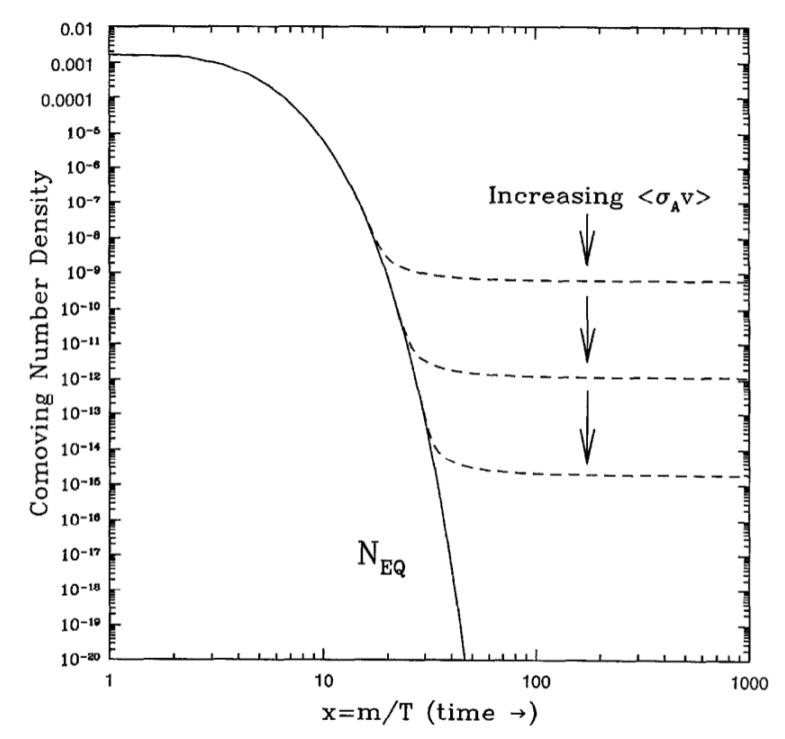
\includegraphics[width=0.6\textwidth]{figs/WIMP_Miracle.jpg}
	\mycaption[WIMP freeze out] {Evolution of the dark matter number density 		as a function of mass over temperature in the universe (proportional to increasing time after the Big Bang). Different assumed annihilation cross-sections $\sigma_{ann}$ lead to differing relic dark matter number densities. Image taken from~\cite{Jungman:1995df}}
	\label{fig:WIMP_Miracle}
\end{figure}  

From calculation of the DM particles abundance, the freeze out temperature is estimated to be $T_{fo} \approx m_{\chi} / 20$. The number density after freeze-out depends strongly on the co-annihilation rate and decreases for larger values of $\left<\sigma_{ann}v\right>$. Assuming \cdm\ description of the Universe evolution, The current relic abundance for DM $\Omega_{\chi} h^2$ can be simplified to:
\begin{equation}
\label{eq:wimp}
\Omega_\chi h^2 \approx \frac{3\times10^{-27}cm^3s^{-1}}{\left<\sigma_{ann}v\right>}.
\end{equation}   

Equation~\ref{eq:wimp} yields that a the co-annihilation cross section is $\sim 10^{-26}$, which is typical for the electroweak scale, where it is expected to find new physics. This great coincidence is called the \textit{The WIMP Miracle}.

In several extension of the SM such as Super Symmetry, a particle candidate with such properties arise naturally. The motivation from cosmology along with the ones from particle physics have promoted the WIMP to be one of the leading classes of DM candidates. 

Over the years many extension and modifications to the WIMP paradigm have been proposed. These modifications include the \textit{inelastic WIMP}~\cite{InelasticIntro}. In this scenario, WIMPs ($\chi_1$) have 3 important additional features:
\begin{itemize}
\item Highly suppressed elastic scattering cross section with nuclei.
\item Second mass state $\chi_2$ havier than $\chi_1$ where $\delta_m$ is of the order of a typical halo WIMP kinetic energy. Generally, $\delta \sim 100$\,keV for weak scale values. 
\item Allowed scattering off of nuclei with an inelastic transition of the dark matter particle, i.e., $\chi_1 + n \rightarrow \chi_2 + n$
\end{itemize}




\section{Dark Matter Detection}
\label{sec:DMDet}

The extensive amount of convincing evidence explained in~\ref{sec:Evidence} lead to a world race towards the detection of DM. There are three main channels to probe DM interaction, a schematic of which is shown in Fig~\ref{fig:detectionScheme}.

\begin{figure}[]
	\centering
	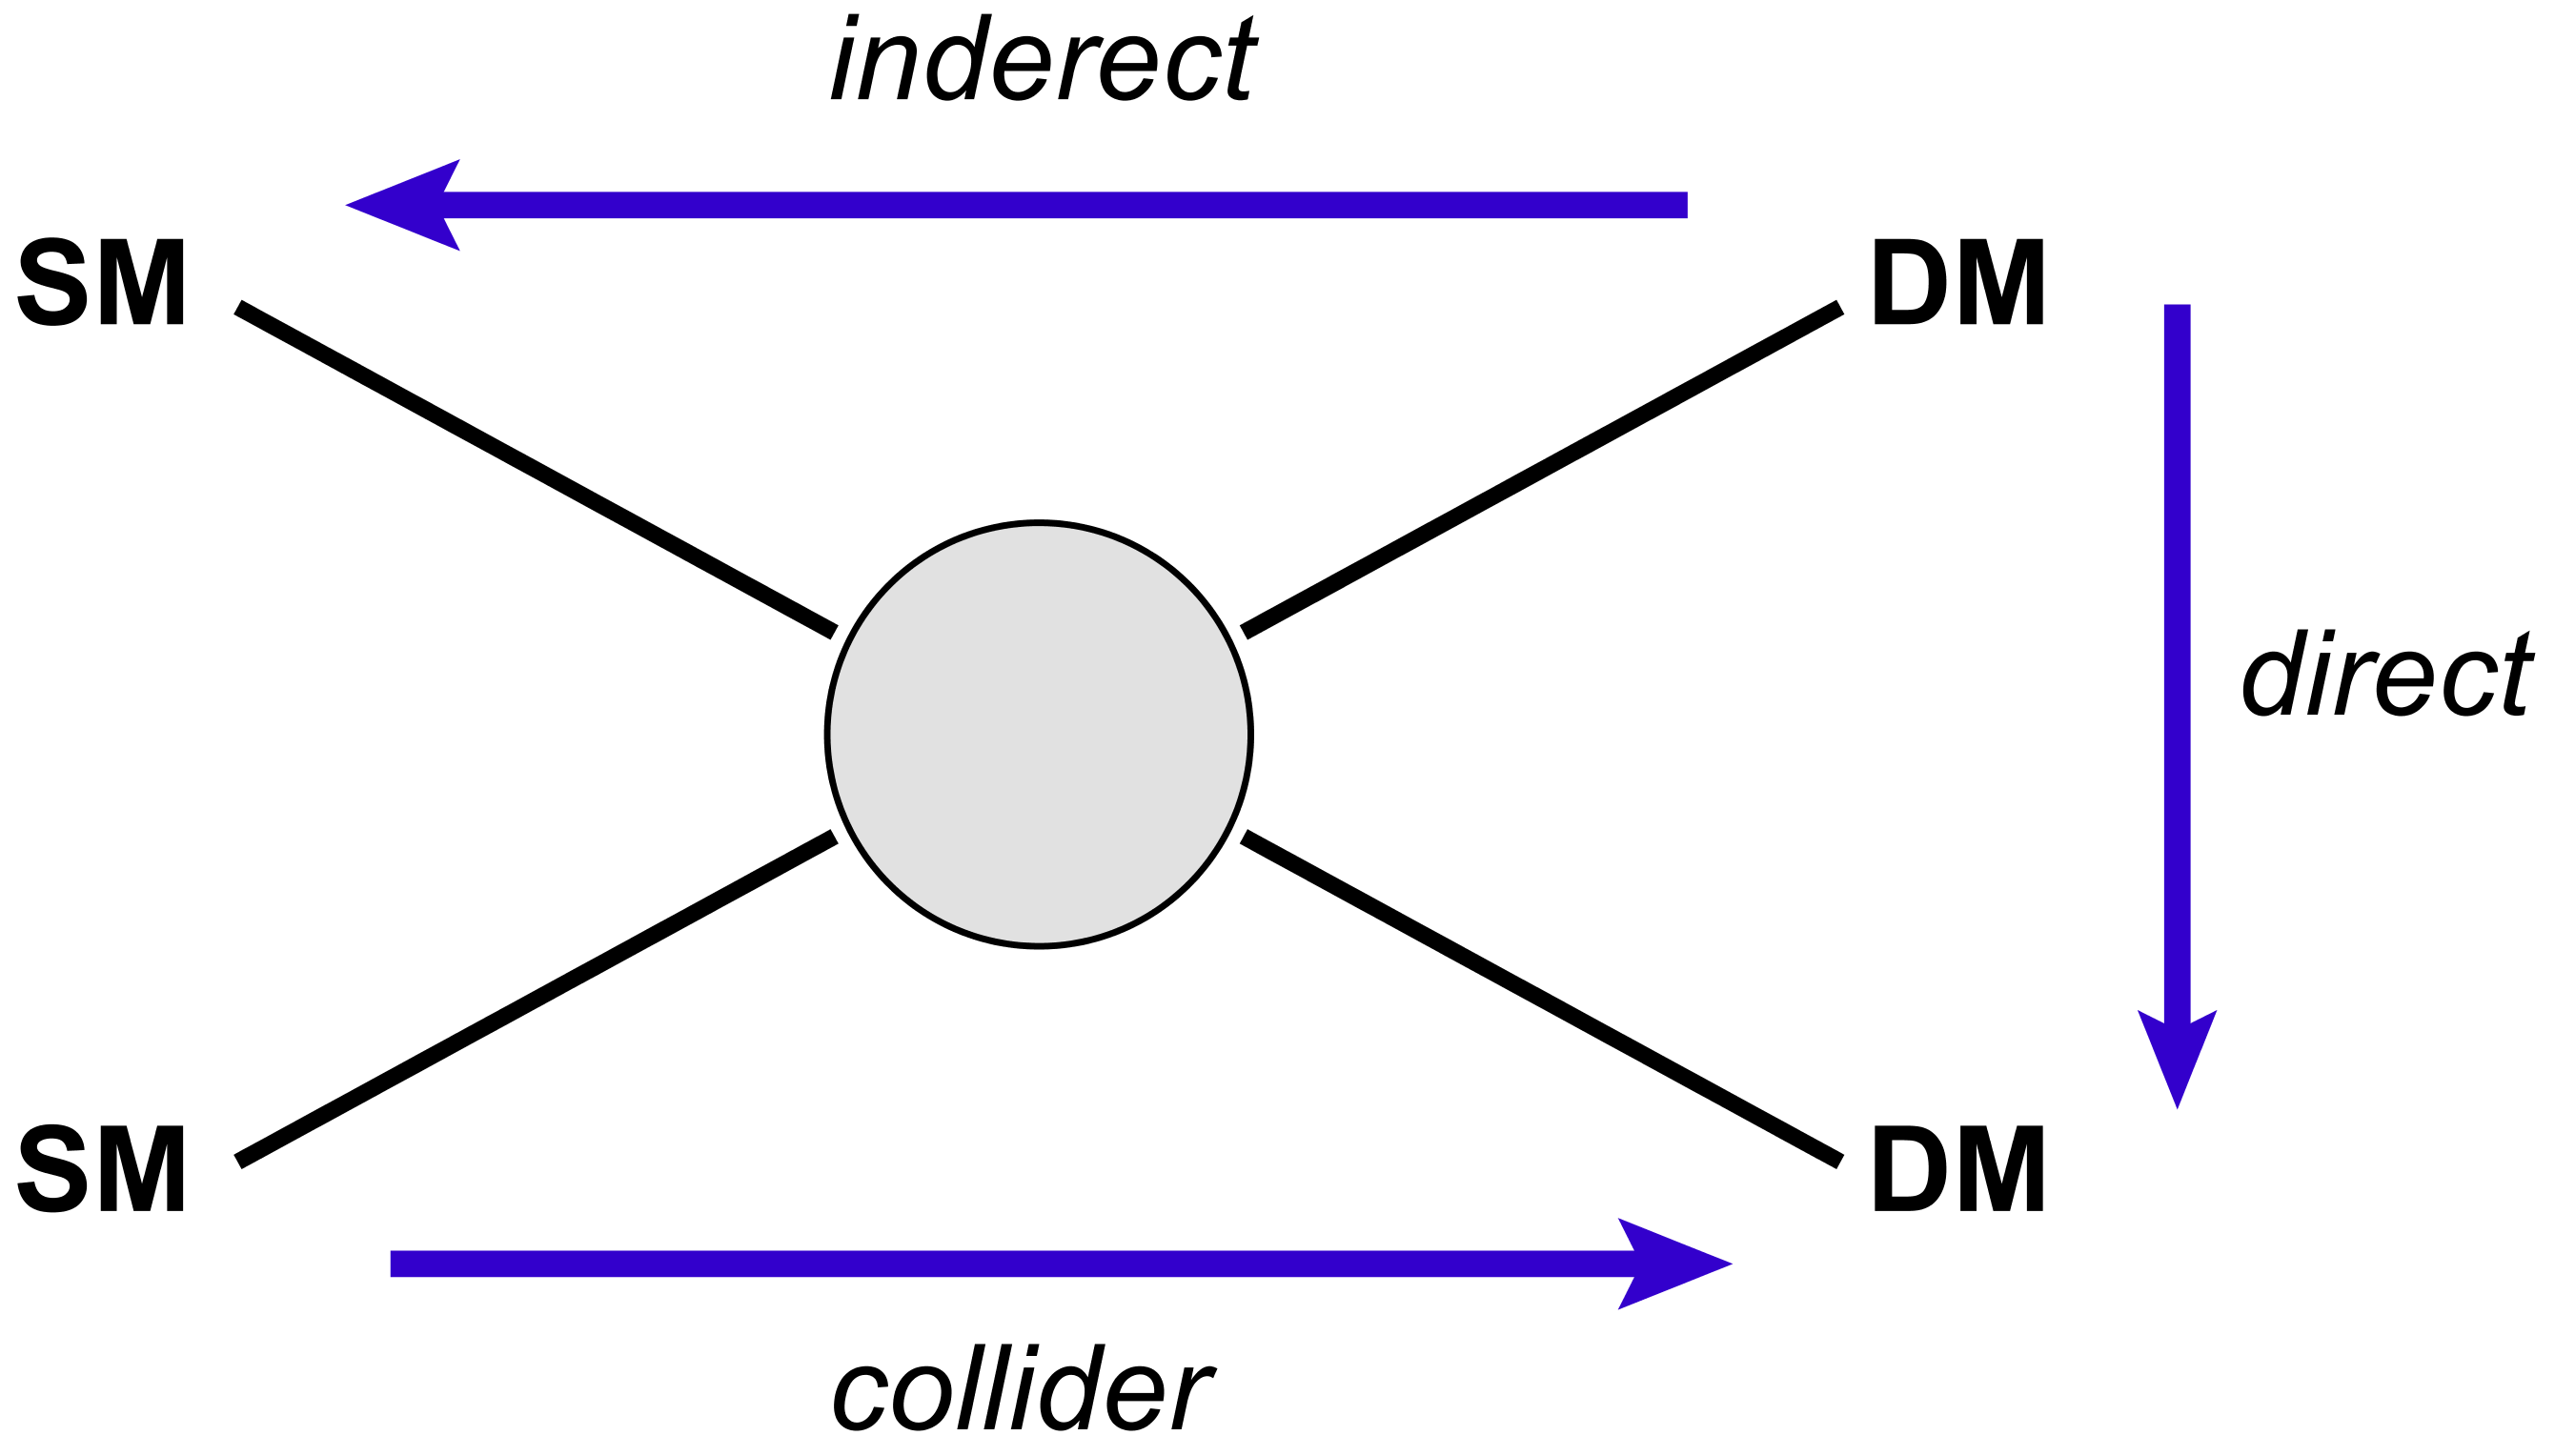
\includegraphics[width=0.6\textwidth]{figs/detection_channels.png}
	\mycaption[DM detection channels] {A schematics of the potential channels for DM detection.}
	\label{fig:detectionScheme}
\end{figure}  

\subsection{Colliders Searches}
\label{subsec:collider}

WIMPS can be produced by the energetic collision of two SM particles (e.g., $q\bar{q}$, $ee^+$). The signature expected for such process include quark jets, leptons, but more importantly missing transverse momentum carried away by the undetectable produced DM particle. So far all searches of colliders have ended up with null results~\ref{fig:ColliderLimit}.  

Even upon detection, the full nature of DM cannot be probed in collider experiment as they cannot prove stability beyond the traveling time in the detector, a key ingredient for WIMPs. Moreover the compression between collider results and direct detection ones, is not trivial, and can be done only in a model dependent way.
\begin{figure}[]
	\centering
	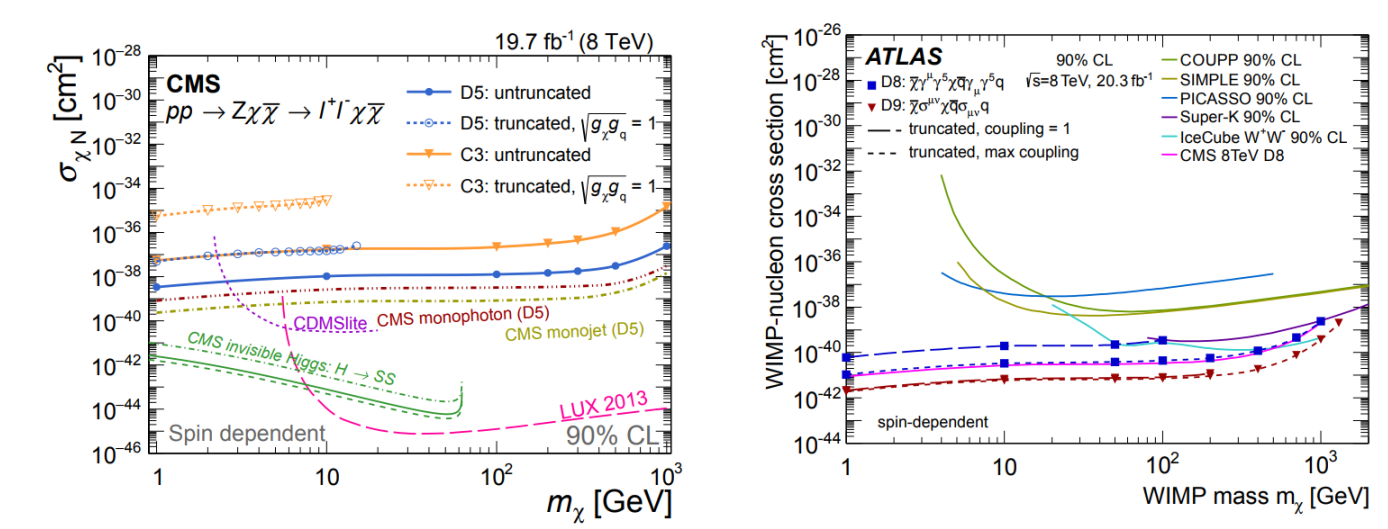
\includegraphics[width=\textwidth]{figs/ColliderLimit.png}
	\mycaption[Limits on DM from the LHC] {90\%CL upper limits on the DM-nucleon scattering cross section, from the monojet, monophoton, and mono-Z searches, as a function of the DM mass.left (right) Spin-independent (spin-dependent) interaction. Several interaction types and dark-matter particle natures are considered~\cite{Lowette:2016orb}.}
	\label{fig:ColliderLimit}
\end{figure}  

\subsection{Indirect Detection Search}
\label{subsec:indirect}
Indirect detection refers to a technique that uses observations
of SM particles which can be created from the co-annihilation or decay of dark matter in our Galaxy and throughout the Universe. The total number of dark-matter particles does not change significantly after freeze-out in the early universe, but their spatial distribution changes considerably during structure formation. 

The signals in indirect searches are SM products of the dark matter annihilation and decay process. most channels result immediately in unstable SM particles which quickly decay and hadronize into stable states. Stable states include photons, neutrinos, electrons and positrons, protons antiprotons, and heavier nuclei and anti-nuclei. For a thorough review on indirect detection searches see~\cite{Conrad:2014tla}.\\

	\textbf{$\gamma$-ray channel}\\

$\gamma$-ray can be produced from WIMP annihilation in various ways: the annihilation into quarks and gauge bosons resulting in a continuous spectrum; direct annihilation to $\gamma$-rays and virtual internal bremsstrahlung resulting in spectral features, which constitute a smoking-gun signal that cannot be explained without DM.

These expected signals are overlaid with background coming from conventional astrophysical sources. In WIMP mass between O(100\,MeV) -- O(100\,GeV), pair-conversion telescopes on satellites (e.g., Fermi Large Area Telescope) are most sensitive. For WIMP mass above $\sim 10$\,GeV Imaging Air Cherenkov Telescopes (e.g., HESS, MAGIC, VERITAS) become more sensitive.\\

\textbf{Charge Cosmic Rays}\\

In this channel the main signature for DM is in the anti-proton and positron flux. As anti-particles are  only produced seldom, even a small addition of WIMP annihilation produced anti-particles is detectable. The signal reveals itself as a rise in the ratio of particle anti-particle flux (e.g., $e/e^+$). Measuring the ratio also reduces the uncertainties of the measurement.  

The leading experiment in this channel is AMS-02 which detected a rise in the positron flux in 2013~\cite{Aguilar:2013qda} and in 2016 released a press note with claims of a signal of WIMPs with mass of 1\,TeV (see Fig.~\ref{fig:AMS}). These results can be explained also by other ways~\cite{Blum:2013zsa} and are not published in a paper yet. \\

\begin{figure}[]
	\centering
	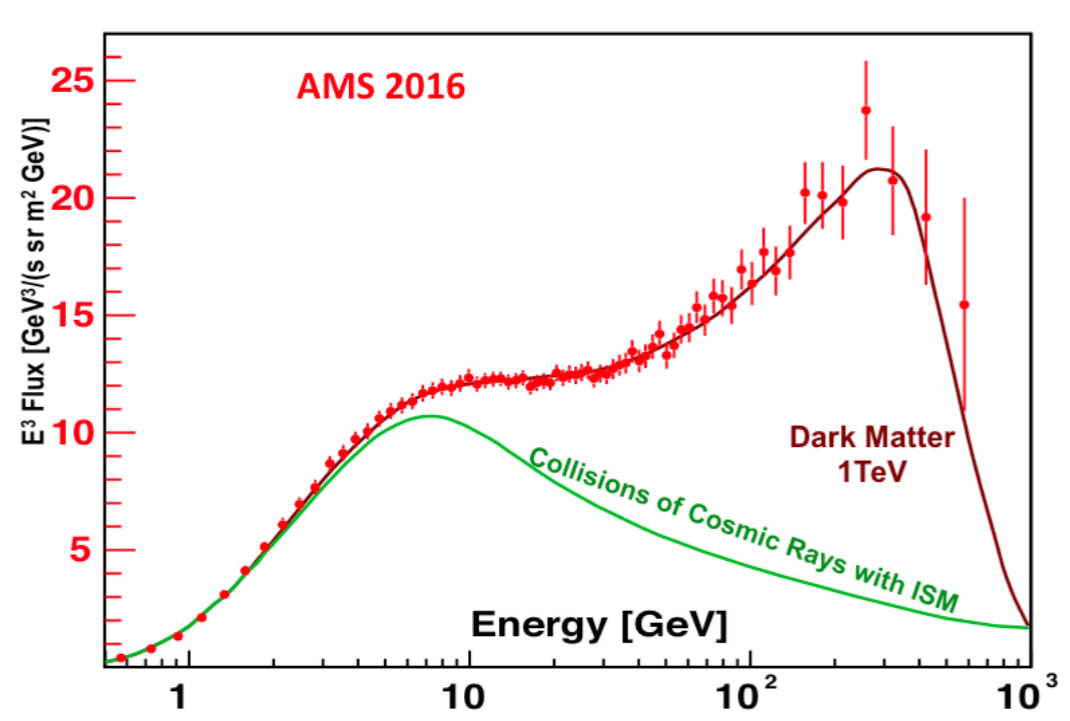
\includegraphics[width=0.8\textwidth]{figs/AMS02.png}
	\mycaption[AMS-02 observetaion of a 1TeV WIMP] { The current AMS positron flux measurement compared with theoretical models. The green line represents the expected flux of positrons from cosmic rays collisions with interstellar material, the red line is the expected spectrum of a 1\,TeV WIMP, and the light red data points are the observed flux.}
	\label{fig:AMS}
\end{figure}  

\textbf{Neutrino Channel}\\

DM can be gravitationally trapped in celestial bodies such as stars and planets. This results in an enhanced DM population near the center of these objects. As a consequence of the increased density the annihilation rate of DM inside stars is substantially larger. All the produced particles will thermalize except for the neutrinos which will escape and can be detected by neutrino detectors such as IceCube~\cite{Achterberg:2006md} and ANTARES~\cite{Collaboration:2011nsa} which sets currently the strongest limits from this channel.

\subsection{Direct Detection Search}
\label{subsec:directdetection}

This search channel refers to measuring on Earth, the interaction between WIMPs and SM particles. Experiments trying to observe WIMP interaction through this channel (e.g., XENON, LUX, ArDM, CDMS and more) are situated in underground laboratories. The various detection strategies as well as relevant calculations are presented in in the following sections.

\section{Interaction Rate}
If WIMPS are moving through Earth, a large number of them, are expected to pass through any terrestrial detector. The rate of interactions per unit mass on a target is:
\begin{equation}
dR = \frac{N_0}{A}\sigma v dn(v),
\end{equation} 
where $A$ is the atomic mass of the target, $\sigma$ is the cross section, $N_0$ is Avogadro number. The differential particle density $dn(v)$ is
\begin{equation}
dn(v) = \frac{\rho_{\chi}}{m_{\chi}*k} f(v,v_E)d^3 v,
\end{equation}
where $v$ is the WIMP velocity in the detector rest frame, $v_E$ is the Earth velocity in the galactic rest frame, and $f(v,v_E)$ is the WIMP velocity distribution usually assumed to be a Maxwell-Boltzmann distribution
\begin{equation}
f(v,v_E) = exp\left(\frac{-(v+v_E)^2}{\sigma_v ^2}\right),
\end{equation} 
where $\sigma_v$ is the WIMP speed dispersion. The normalization factor $k$ is defined such that
\begin{equation}
k = \int_0^{2\pi}d\phi \int_{-1}^1d(\cos(\theta)) \int_0^{v_{esc}} exp\left(\frac{-(v+v_E)^2}{\sigma_v ^2}\right),
\end{equation}
yielding,
\begin{equation}
\int_0^{v_{esc}} dn \equiv \frac{\rho_\chi}{m_\chi} 
\end{equation}
where $v_{esc}$ is the  local galactic escape velocity. Standard values for the velocity distribution parameters are:
\begin{equation}
\sigma_v = 230\mathrm{km/s}, \qquad v_{esc} = 600\mathrm{km/s} \rightarrow k \approx (\pi \sigma_v^2)^{3/2}
\end{equation} 

The recoil energy of a nucleus with mass $m_N$ stroke by a DM particle with kinetic energy $E = \frac{1}{2}M_\chi v^2$ scattered at an angle $\theta$ is: $E_R = E_0r(1-\cos(\theta))/2$ where $r \equiv \frac{4M_\chi M_N}{(M_\chi + M_N)^2}$ and $E_0=\frac{1}{2}M_\chi\sigma_v^2$. Assuming isotropic scattering the recoils are distributed uniformly in $E_R$, where $0 \leq E_R \leq E_0 r$; therefore
\begin{equation}
\frac{dR}{dE_R} = \int_{E_{min}}^{E_{max}} \frac{1}{E_0 r}dR(E) = \frac{1}{E_0r}\int_{v{min}}^{v_{max}}\frac{\sigma^2}{v^2}dR(v),
\end{equation} 
where $E_{min}$ is the smallest possible recoil energy and $v_{min}$ is its corresponding velocity. For a more comprehensive treatment of the WIMP interaction rate see~\cite{LEWIN}. In Fig.~\ref{fig:interactionRate}, is an example of the interaction rate for various elements.

\begin{figure}[t!]
	\centering
	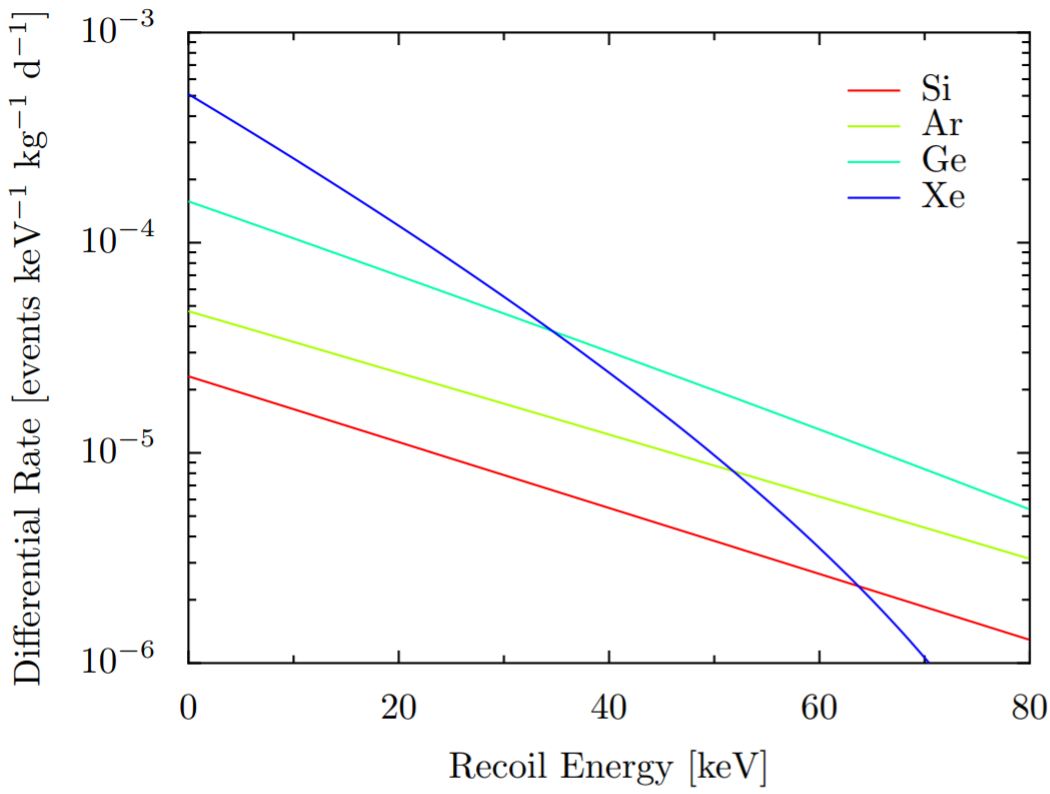
\includegraphics[width=0.8\textwidth]{figs/EventRate.png}
	\mycaption[Differential event rate for various elements.]{ Expected differential recoil spectra from WIMP-nucleon scattering in different
target materials, for a WIMP mass of $m_\chi= 100$\,GeV, assuming SI cross section of $\sigma_\chi = 10^{-44} \mathrm{cm}^2$}
	\label{fig:interactionRate}
\end{figure}



\subsection{WIMP Nucleus Interaction Cross Section}
\label{subsubsec:WIMP_CS}

WIMPs are charged under $SU(2)_{weak}$, hence they will interact with matter via weak-interactions. The cross section for zero momentum transfer is traditionally modeled as: $\sigma_0 = 4G^2_F\mu_N^2C$, where $G_F = 1.1\times 10^{-5}\,GeV/(\hslash c)^3$ is the Fermi constant, $\mu_N$ is the WIMP-target reduced mass, and $C$ is an enhancement factor which is determined by the nature of the WIMP. $C$ is different for different types of interactions. The \textit{standard} interaction types treated in direct detection experiments are the spin-dependent (SD) and spin-independent (SI) which are reviewed in this section. For a discussion on other types of motivated interactions (e.g., spin-orbit) see Sec~\ref{sec:intro_EFT}.

For the SI case the enhancement factor is modeled as:
\begin{equation}
C_{SI} = \frac{1}{\pi G_F^2}[Zf_p + (A-Z)f_n]^2,
\end{equation} 
where $f_p$ and $f_n$ are the effective WIMP-proton, WIMP-neutron coupling respectively. This type of interactions grows as $A^2$, and favors heavy targets. This type of interaction can appear due to isoscalar currents.
\begin{equation}
\mathcal{L} \supset \alpha_q^S \bar{\chi} \chi \bar{q}q + \alpha_q^V\bar{\chi}\gamma_\mu\chi\bar{q}\gamma^\mu q.  
\end{equation}

In the SD case, the scattering amplitude changes sign with the spin orientation; hence, only isotopes with odd number of protons  or neutrons can be used for detection. The enhancement factor is modeled as:
\begin{equation}
C_{SD} = \frac{8}{\pi J}[a_p\left<S_p\right> + a_n\left<s_n\right>]J(J+1).
\end{equation}  
$a_p$ and $a_n$ are the WIMP-proton and WIMP-neutron effective coupling respectively,$\left<S_p\right>$ and  $\left<S_n\right>$ are the proton and neutron spin, and $J$ is the total nuclear spin. This type of interaction can appear due to isovector currents such as:
\begin{equation}
\mathcal{L} \supset \alpha_q(\bar{\chi}\gamma_\mu\gamma_5\chi)(\bar{q}\gamma^\mu\gamma_5q)
\end{equation}
\subsection{Form Factors}

At high momentum transfer, the inverse nuclear size becomes comparable to the momentum transfer (few hundred keVs), causing the cross section to drop due to the loss of coherence. To account for this effect, nuclear form factors, which are essentially the Fourier transform of the nucleon density function are introduced ($F(q)$). Usually the form factors are parametrized as a function of  the dimensionless quantity $qr_n$, where $r_n$ is the nuclear radius. The cross section can be separated into two parts:
\begin{equation}
\sigma(qr_n) = \sigma_0F^2(qr_n),
\end{equation}
where $\sigma_0$ is the zero-momentum transfer cross section, and $F(qr_n$ is the form factor, containing all momentum-transfer dependency. Much study has been conducted on the exact parametrization of the form factors~\cite{Feldstein:2009tr}; however for low momentum transfer the effect of the different parametrization is negligible. 

Finally the total event rate as a function of recoil-energy is given by:
\begin{equation}
\frac{dR}{dE_R} = \frac{\rho_\chi}{M_TM_\chi}\int_{v>v_{min}}^{v_{esc}}d^3v\cdot \frac{d\sigma_i}{dE_R}\cdot F_i^2(q^2)f(v,v_E)v
\end{equation} 
Where the astrophysical input are incorporated in the first and last terms. The particle and nuclear physics is incorporated in the $\sigma_i$ and $F^2_i(q^2)$ are the the cross section and form factor for interaction type $i$ respectively.
\section{Effective Field Theory Approach for WIMP-Nucleolus Scattering}
\label{sec:intro_EFT}

The traditional approach for calculating the WIMP-nucleon scattering rate, has been to take only leading-order terms in a WIMP-nucleon effective field theory (EFT) with a very simple treatment of nuclear structure (as explained in Sec.~\ref{subsubsec:WIMP_CS}). This leads to two main types of interactions, which are commonly labelled SI and SD. However, in recent years many authors have pointed out that in certain theories these interactions may be suppressed or nonexistent, and that otherwise subleading interactions may dominate the scattering process~\cite{Chang:2009yt}. To account for this possibility in a systematic way, a more sophisticated EFT approach has been developed ~\cite{Fitzpatrick:2012ib,Anand:MathTools,Fitzpatrick:MathTools}. In the new approach, an effective Lagrangian describing the WIMP-nucleus interaction is constructed, taking into account all Galilean-invariant operators up to second order in the momentum exchange. This framework introduces new operators associated with different types of nuclear responses, along with the standard SI and SD ones, resulting in a set of 14 operators $\mathcal{O}_i$ which may couple independently to protons and neutrons. In Eqs. (\ref{eq:OpDef}) I list these operators following the convention from~\cite{Anand:MathTools}. The operators depend explicitly on four linearly independent quantities: $\vec{v}_{elastic}^{\perp} \equiv \vec{v} + \frac{\vec{q}}{2\mu_N} $; the relative perpendicular velocity between the WIMP and the nucleon; $\vec{q}$, the momentum transferred in the scattering event; and $\vec{S}_\chi$ and $\vec{S}_N$, the WIMP and nucleon spins. $\mathcal{O}_2$ is not considered here as it cannot be obtained from a relativistic operator at leading order.
%

\begingroup
\belowdisplayskip=0pt
\begin{align*}
\begin{split} 
&\mathcal{O}_1 = 1_{\chi} 1_N  \\
%&\mathcal{O}_2 = (v^{\perp})^2 \\
&\mathcal{O}_3 = i\vec{S}_N\cdot (\frac{\vec{q}}{m_N}\times\vec{v}_{el}^{\perp}) \\
&\mathcal{O}_4 = \vec{S}_{\chi}\cdot \vec{S}_N \\
&\mathcal{O}_5 = i\vec{S}_{\chi}\cdot (\frac{\vec{q}}{m_N}\times\vec{v}_{el}^{\perp}) \\
&\mathcal{O}_6 = (\vec{S}_{\chi} \cdot \frac{\vec{q}}{m_N})(\vec{S}_N \cdot \frac{\vec{q}}{m_N}) \\
&\mathcal{O}_7 = \vec{S}_N \cdot \vec{v}_{el}^{\perp} \\
&\mathcal{O}_8 = \vec{S}_{\chi} \cdot \vec{v}_{el}^{\perp}  \\
\end{split}
\begin{split}
&\mathcal{O}_9 = i\vec{S}_{\chi} \cdot(\vec{S}_N \times \frac{\vec{q}}{m_N}) \\
&\mathcal{O}_{10} = i\vec{S}_N \cdot (\frac{\vec{q}}{m_N}) \\
&\mathcal{O}_{11} = i\vec{S}_{\chi} \cdot (\frac{\vec{q}}{m_N}) \\
&\mathcal{O}_{12} = \vec{S}_\chi \cdot (\vec{S}_N \times \vec{v}_{el}^{\perp}) \\
&\mathcal{O}_{13} = i(\vec{S}\chi \cdot \vec{v}_{el}^{\perp})(\vec{S}_N \cdot \frac{\vec{q}}{m_N})\\
&\mathcal{O}_{14} = i(\vec{S}_\chi \cdot \frac{\vec{q}}{m_N})(\vec{S}_N \cdot \vec{v}_{el}^{\perp}) \\
\end{split}
\end{align*}
\endgroup
\begingroup
\abovedisplayskip=0pt
\begin{align}
&\mathcal{O}_{15} = -(\vec{S}_\chi \cdot \frac{\vec{q}}{m_N})\left[(\vec{S}_N \times \vec{v}_{el}^{\perp})\cdot \frac{\vec{q}}{m_N}\right]
\label{eq:OpDef}
\end{align}
\endgroup

Unlike the commonly studied types of interaction (SI and SD), which are not suppressed when $\vec{q} \rightarrow 0$ and for which the scattering rate on nucleons is expected to be largest for low energy nuclear recoils, some of the new EFT operators depend explicitly on $\vec{q}$ and so their interaction cross section is suppressed for low momentum transfers. Consequently, their scattering rate peaks at nonzero nuclear recoil energy. For sufficiently high WIMP masses, this may occur above typical analysis energy range, which usually have an upper range of around $ 43\,\keVr$ (nuclear recoil equivalent
energy) since they are designed to search the exponentially falling recoil spectra expected for SI and SD interactions (see Fig.~\ref{fig:EFTdrde}).High energy nuclear recoils (NR), therefore, remain unexplored in many experiments.

	    Another typical assumption that can be relaxed is that WIMPs should scatter elastically with nuclei. There are dark matter models in which the incoming and outgoing WIMPs have different mass states~\cite{InelasticIntro} separated by a keV-scale splitting. In the case where the outgoing state is more massive than the incoming state, the cross section for low recoil energies can again be suppressed, this time by scattering kinematics. Recently an inelastic adaptation of the EFT operator framework discussed above was developed~\cite{InelasticMath}. In this case the operators presented in Eqs.~\ref{eq:OpDef} are modified such that $\vec{v}^{\perp}_{inelastic} = \vec{v}^{\perp}_{elastic} +\frac{\delta_m}{\vert{\vec{q}}\vert^2}\vec{q}$, where $\delta_m = $ is the mass splitting of the two WIMP states. In this paradigm the minimum momentum transfer for an interaction to occur is given by:
\begin{equation}
  v_\mathrm{min}/c = \frac{1}{\sqrt{2 m_N E_R}} \left|\frac{m_N E_R}{\mu_N} + \delta_m\right|,
\end{equation}
where $\mu_N$ is the WIMP-nucleon reduced mass.



\section{Direct Detection Strategies}
\label{sec:detStrtegies}

The expected WIMP interaction flux and interaction types and rates, as well as the expected flux (explained above) are used as to design any instrument aiming at the detection of WIMP scattering from a target nuclei (direct detection). The detector must have a low threshold for NR O(1-10)\,keV as most WIMP paradigm yields an exponential decay of the recoil spectrum. Hence a lower threshold yields a large increase in sensitivity. The expected total interaction rate in a detector is very low; therefore the detector should have low background.

%TODO add background sources here

The main background source for WIMP detection is in the form of ER, and can be divided into two: external and internal background. External background refers to any particle entering the detector from outside and interacting within the detector. $\gamma$ and $\mu$ are the main types of particle which can penetrate the detector. Internal background refers to radioactive isotopes of the detector materials ($^{39}$Ar) or impurities ($^{222}Rn$ and $^{85}$Kr).
In addition neutrons or neutrinos can also induce NR background which is currently irreducible. 


Many efforts are devoted for reducing ER background, focusing on decreasing the radioactive contaminations, in addition to stating the detector in a low background environment. Most detectors are situated in an underground facility to reduce muon flux from cosmic rays (see Fig.~\ref{fig:MuonRed}). Additionally, if the detector has the ability to discriminate between NR (signal) and ER (background) it will it will increase its detection sensitivity, as most background comes from $\gamma$-rays and $\beta$ decays will be rejected. Because the event rate grows with target volume, the larger the number of nuclei is, the larger is the detector sensitivity, this can compensate for bigger background rates. Finally would the detector have the ability to identify special features of WIMPS such as interaction types, and the directionality of the the incoming WIMP, it will have a clearer signature of WIMP detection.

\begin{figure}[]
	\centering
	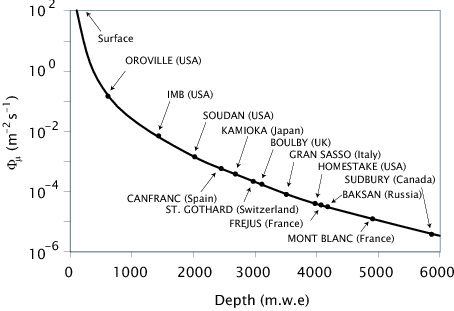
\includegraphics[width=0.8\textwidth]{figs/muones.png}
	\mycaption[Muon flux in underground facilities]{ The muon flux as a function of underground facility depth measured in meter water equivalent. }
	\label{fig:MuonRed}
\end{figure}

The energy deposited in a material by any interacting particle, can be measured by three excitation channels: scintillation, ionization, and heat (phonons). Different detectors use different excitation channels; scintillators based experiments use light detectors to detect the scintillation lights (e.g., DAMA/LIBRE), Germanium based detectors usually use the ionization channel (e.g., CoGeNT) and superconductor based experiment detect heat (e.g., CRESST). Most leading experiments measure two of the excitation channel (e.g., XENON measuring scintillation and ionization). The measurement of two excitation channels gives a better ability to discriminate signal to background. The discrimination parameter is usually the ratio between the two channels.  

Past and present representative experiments of WIMP direct detection and the detection method they use are shown in Fig.~\ref{fig:det_strategy}. In the next section I focused on Liquid-Noble detectors, mainly on XENON based detectors.  

\begin{figure}[]
	\centering
	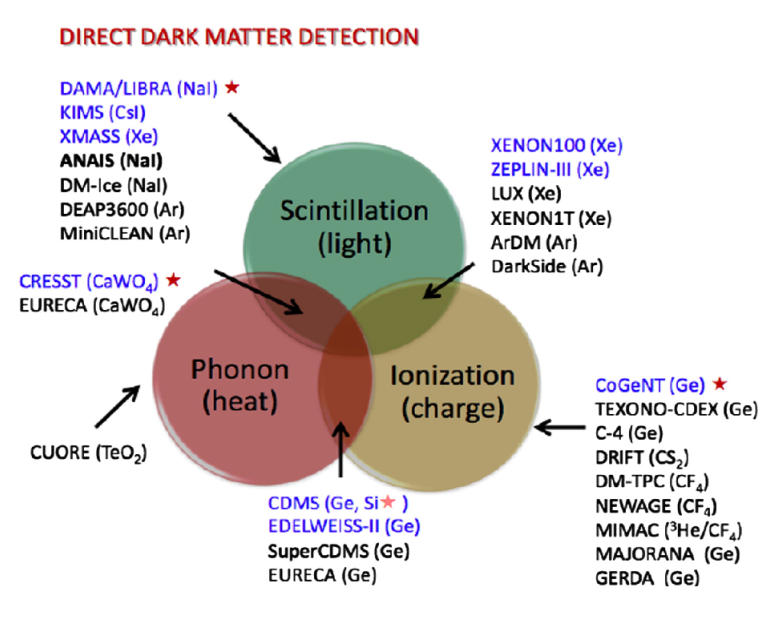
\includegraphics[width=0.8\textwidth]{figs/DetChannels.png}
	\mycaption[Excitation detection channels.]{ Direct detection experiments classified by their detection strategies.}
	\label{fig:det_strategy}
\end{figure}

\section{Nobel Liquid Detectors}
\label{sec:liquidDet}

The most sensitive DM direct detection detectors currently are based on Liquid Noble elements, mainly Xenon and Argon. The excitation channels these detectors utilize are the scintillation and ionization. The strategy these detectors exploit for lowering the background rates is the self-shielding of the target materials. PMT arrays deployed in the liquid xenon (LXe) or liquid argon (LAr) detects the photons from the scintillation. Extracting the ionization electrons using an electric field allows ionization measurement. The ionization to scintillation ratio and the pulse shape can be used as discriminator parameters between signal (NR) and background (ER). The low concentration of radioactive isotopes results in an inner volume practically free of electromagnetic background. Liquid noble detectors are divided into two; liquid only detectors (single phase) and liquid and gas detectors (dual phase).

\subsection{Single Phase Detectors}
\label{sec:singlePhase}
 
Single phase detectors fully exploit the self-shielding properties of LXe and LAr to create a low background inner volume. These experiment usually relay on light detectors immersed in the liquid target. The position reconstruction of an interaction is obtained by the observed light hit pattern and its resolution depends on the photodetector size. The main advantage of these detectors is their simplicity. Since no ionization measure is used, the complexity in adding high voltage and cathode-anode-grid systems is avoided. The main disadvantage is that less information is known about each interaction event and the discrimination between ER and NR is less efficient. 

An example of a single phase LXe detectors is the XMASS detector, positioned in the Kamioka observatory in Japan. It is a spherical detector holding 830\,kg of LXe  surrounded by 642 PMTs. The detector is deployed in a 10\,ton water tank to reduce background. XMASS have excluded a cross section of $1.5\times 10^{-43}$\,cm$^2$ for a 100\,GeV WIMP with an exposure of 292 days~\cite{Hiraide:2016ryf}. An example for future LAr single phase detector is the DEAP experiment located in SNOLab underground facility. The LAr pulse shape discrimination that will be used to enhance the expected sensitivity. The detector is expected to hold more than 1-tonne of LAr with background expectation of less than $0.3$ event/year. 
 
\subsection{Dual Phase Detectors}
\label{sec:dualPhase}

Dual phase detectors rely on time projection chamber (TPC) technique, exploiting both scintillation and ionization channels. The scintillation photons are detected like in the single phase detectors usually using PMTs. The ionization electrons drifts in the liquid due to an external electric field and extracted to the gas phase using a stronger electric field, and generate proportional scintillation. The ratio of the two signals is used as a discriminator parameter, as ER produces a higher ionizion signal compared to NR. a full 3D position reconstruction is achieved using the hit pattern of the proportional scintillation and the time difference between the two signals. A more detailed desciption of the XENON experiment TPC can be found in~\ref{sec:xenonProg}.

The leading dual phase LXe collaborations are LUX~\cite{Akerib:2012ys} PANDAX~\cite{Cao:2014jsa} and XENON1T~\cite{Aprile:2017aty} Currently XENON1T sets the most stringent limit for the SI interaction~\cite{Xenon1TResults}. LAr have an additional advantage using  pulse shape discrimination techniques. The main disadventage of LAr is the low PMT efficiency for argone scintillation light. The most common way to increase the detection efficiency is by coating the PMT with a wavelength shifter. Amongst the leading LAr programs are WArP~\cite{Zani:2014lea}, ArDM~\cite{Rubbia:2005ge}, and DarkSide~\cite{Alexander:2013hia}  

%%======
\section{Non Linear Emission of Radiation in Liquid Xenon}
\label{sec:intro_superradiance}
As explained in Sec.~\ref{sec:detStrtegies}, in LXe and LAR based experiments the exact properties (time and spatial) of the scintillation and ionization responses to all types of interaction must be well quantified and understood. Mainly, much research has been focused on the scintilation and ionization responses of LXe to events with recoil energy as low as <O(10\,keV)~\cite{Manzur:2009hp,Aprile:2012an,Baudis:2013cca,Akerib:2016mzi}.
Specifically the reconstruction of the directionality of recoil nuclei or electrons is of great interest to DM direct detection experiments. Better understanding of these properties may help to reduce background dramatically, both by detecting the direction of the incoming particle, and by better discriminating ER and NR. 

A particle interacting within the LXe media, forms a cloud of excited and ionized states with typical length of 100~nm. 
The excited Xe ($Xe^*$) combines with other Xe atoms to form an excited dimer state (excimer) when they decay to ground state they emit light. 
\begin{equation} \label{eq:XeSci1}
 Xe^*+Xe \rightarrow Xe^*_2 \rightarrow 2Xe + h \nu , 
\end{equation}
The electrons emitted from the ionization can recombine with a surrounding atom, this process of recombination provides another possibility to produce excimers,
\begin{equation} \label{eq:XeSci2}
\begin{split}
  &Xe^{+} + Xe \rightarrow Xe^{+}_2 \\
  &Xe^{+}_2 + e^{-}  \rightarrow Xe^{**} \\
  &Xe^{**}   \rightarrow Xe^* + heat .\\
  \end{split}
\end{equation}  
Once $Xe^*$ is produced it adds to the scintillation process explained in~\ref{eq:XeSci1}. There are two types of $Xe^*_2$ excimer states, 
singlet and triplet, with lifetime of $\sim3$ ns and $\sim25$ ns respectively. The wavelength emitted by these states is between (175-180)~nm 
which is lower then the lowest excitation of xenon, and therefore travel through it to reach a photo-detector situated outside the LXe. In LAr the same process happens however the lifetime of the singlet ($\sim7$\,ns) and triplet($\sim1600$\,ns) are different. Because the ratio of singlets to triplets is different for ER and NR this is used for better discrimination ("pulse shape discrimination")~\cite{Lippincott:2008ad}.

Several existing and proposed experiments such as DRIFT-II~\cite{Muna:2007zz}, DMTPC~\cite{Deaconu:2017vam}, NEWAGE~\cite{Yakabe:2016pjh} and MIMAC~\cite{Riffard:2016mgw}, exploit recoil direction properties. These experiments are using dilute gas in which the ionization tracks extend to a few millimeters. However, in LXe the track length is estimated to be O(100nm). Moreover the topology of the excimers clouds is represented by a complex structure of branches which are formed by secondary recoils~\cite{Chepel:2012sj}. These two different properties, track length and structure, makes it highly difficult if not impossible to construct directionality in a LXe experiment. Therefore, a different approach for directionality measurement needs to be adopted for DM LXe based experiments.

The phenomena of an isolated particle in an excited state undergoing a transition to its ground state (i.e. spontaneous decay) as a result of the vacuum electromagnetic field  is well described in the theory of quantum electrodynamics. This theory is applicable for an ensemble of particles only when the particles interact with the vacuum electromagnetic field separately. In this case the time distribution of emitted light will follow an exponential law. The characteristic time, $\tau_{sp}$, of a single particle to radiate is equal to the the reciprocal of the transition rate $\Gamma$ from the initially excited level. The radiation pattern in this case is isotropic in its nature, see Fig.~\ref{fig:emissionType}a. 

These radiation properties are significantly different when the radiating particles are dense enough. In this case the collective radiation from  the ensemble is different than the sum of all particles radiating. This phenomena was first postulated by Dicke~\cite{DickeSR} in 1954 and was first measured in Xe by Rosenberger in 1965~\cite{FirstMeasure}. In his research the radiation decay time from a two level atomic system was considered and expected to be dependent on the number of radiating particles N. This type of emission is referred as superradiance. This phenomena is due to interaction of the radiating particles with each other via a common electromagnetic radiation field, which results in a correlation between the atomic dipole moment. This correlation leads to a macroscopic optical polarization proportional to N. Hence the radiation intensity is proportional to $N^2$, leading to a pulsed radiation with duration proportional to $1/N$, see Fig~\ref{fig:emissionType}b. The phenomena of superradiance has been studied extensively since see~\cite{Gross1982301,benedict1996super}  
\begin{figure}[t!]
	\centering
	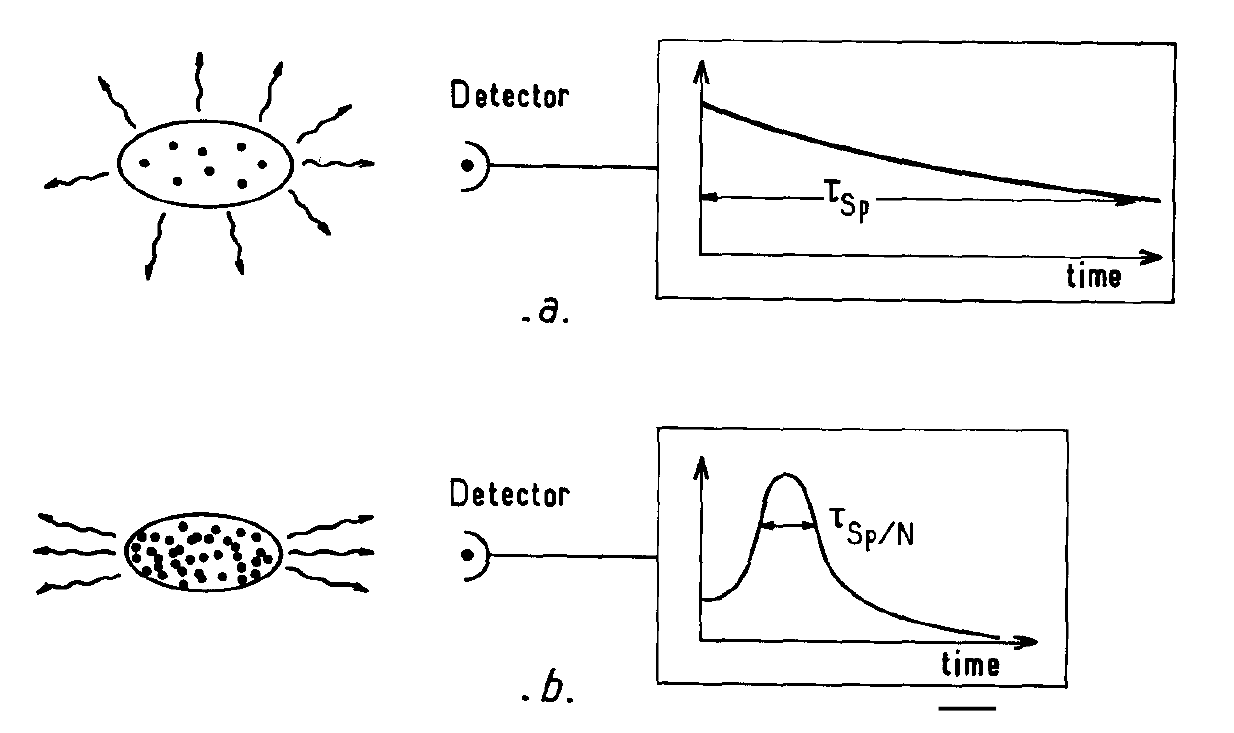
\includegraphics[width=0.8\textwidth]{figs/emissionTypes.png}
	\mycaption[Comparison between ordinary fluorescence and superradiance.]{Comparison between ordinary fluorescence and superradiance. (a) In ordinary fluorescence, where each atom (or molecule) interacts independently with the vacuum electromagnetic field, the intensity
decays exponentially (with time constant $\tau_{sp}$), with an isotropic directional distribution. (b) Superradiance is highly directional and its duration is of order $\tau_{sp}$/N, where N is the number of radiators in the sample. Figure from~\cite{Gross1982301} }
	\label{fig:emissionType}
\end{figure}


An effective self-induction of correlations between dipole moments is a necessary condition for a particles to exhibit a \superradiance\ emission. The conditions for this to occur are very different than the ones of regular fluorescence. The characteristic time of \superradiance\ emission to happen, $\tau_c \sim 1/N $ must be shorter the relaxation time of the atomic dipole moment, $\tau_d$. It also has to be shorter then $\tau_{sp}$, however in most cases, $\tau_{d}$ is smaller than $\tau_{sp}$, hence this is a more stringent condition. Notice that unlike inverse population that happens in lasers, which occurs due to an external "pump", the correlation build-up between the radiating particles in \superradiance\ happens spontaneously in the course of emission process.

The \superradiance\ emission pattern depends greatly on the geometrical configuration of the atomic system. The relevant quantities affecting the  different behaviors are the de-excitation wavelength ($\lambda$) and linear the size of the system (L). There are three different scenarios: $L^3<<\lambda^3$ ; $L \gtrsim \lambda$; $L>>\lambda$. In the first case, a system of radiating particles with linear size much smaller than the wavelength, the system will emit a pulse in an arbitrary direction with a maximal intensity of $I \sim N^2$. In the second case the linear size of the system is comparable to the wavelength , however the distance between 2 radiating particles is still smaller than the wavelength, the system will emit most of its energy into a small solid angle in the direction of the greater dimension of the system. This directionality is caused by the growing interference of the emitted photons. The particles will start emitting isotropic spontaneous emission, and gradually will grow correlations between the atomic dipole via the radiation field. The third case is the case of classical standard emission. 
        








\section{The XENON Program}
\label{sec:xenonProg}

The XENON program for DM searches, is a phases program using LXe detectors to measure the scattering of DM of xenon nuclei. In each phase the mass of the detector increase by roughly an order of magnitude, starting from 10\,kg in the first phase, and ending with 7\,tonne in the last. The program operates the detectors at the Laboratori Nazionali del Gran Sasso (LNGS) in Italy. Under an average depth of 3600 m water equivalent, the cosmic muon
flux is suppressed by six orders of magnitude with respect to sea level (see Fig.~\ref{fig:MuonRed}). The time line for all phases, as well as their properties and sensitivities are presented in Fig.~\ref{fig:XenonProg}.

The XENON detectors are dual phase (liquid-gas) TPCs, with simultaneous
detection of the Xe scintillation light (S1) at the few keV level, and ionization (S2) at the single electron level. The ratio S2/S1 produced by a WIMP (or neutron) interaction is different from that produced by an electromagnetic interaction, allowing a very efficient particle identification.

The ultra low background has been achieved by: careful selection of the materials; the xenon self-shielding capabilities as well as water shielding in advance phases; and selecting data only from a fiducial volume (FV) located at the center of the detector.

A short summary on each phase and its upgrade from previous phase is presented here, the main concepts of the XENON TPC are explained using XENON100 as an example in Sec.~\ref{sec:xe100}.


\begin{figure}[t!]
	\centering
	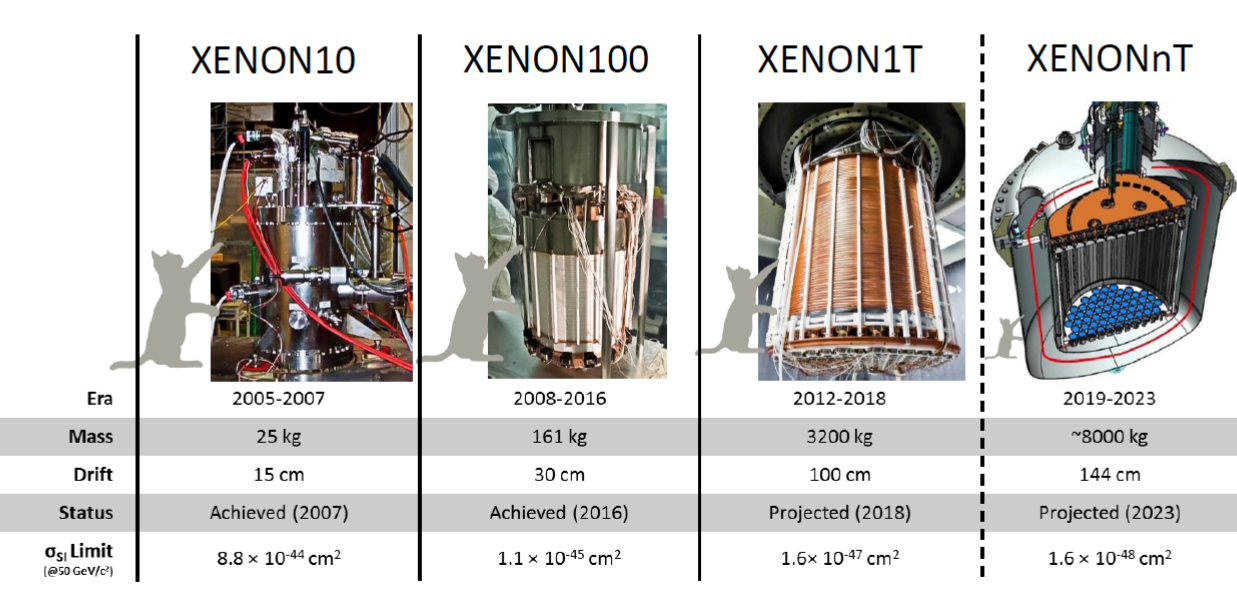
\includegraphics[width=0.95\textwidth]{figs/XePhases.png}
	\mycaption[The XENON Program detectors]{The timeline of the four phases of the XENON program}
	\label{fig:XenonProg}
\end{figure}


\subsection{XENON10}
\label{sec:xe10}
The first phase was the XENON10 detector a cylinder $\sim 20$\,cm diameter and $20$\,cm length, holding 25\,kg of xenon (10\,kg in the FV). The detector was operating mainly as a prototype for the larger detectors to come. It was operating between the years 2005 and 2007, achieving an exclusion limit of $\sigma_{SI} = 8.8 \times 10^{-44}$\,cm$^2$ for a 50\,GeV WIMP~\cite{Angle:2007uj}.

\subsection{XENON100}
\label{sec:xe100}
The second phase was the XENON100 detector a cylindrical $\sim 40$\,cm diameter and $40$\,cm length hosting 161\,kg of LXe, of which 62\,kg function as the active target and 34\,kg as the FV. The detector uses of a total of 178 1-inch square Hamamatsu R8520-AL PMTs employed in two arrays, one in the gas phase at the top of the TPC, and the other at the bottom, immersed in the LXe~\cite{xe100_instr2012}.

A particle interacting with the LXe deposits energy that creates both
prompt scintillation (S1) and delayed proportional scintillation (S2) both finally producing vacuum ultra violet (VUV) 178\,nm photons. The photons are detected using the two PMT arrays. The S2 signal is produced by ionization electrons, drifted in an electric field of $530$V/cm towards the liquid-gas interface, where they are extracted to the gas phase using a stronger electric field of $\sim12$kV/cm in which the proportional scintillation occurs. 
The spatial distribution of the S2 signal on the top PMT array, together with the time difference between S1 and S2 signals, provide respectively $x$-$y$ and $z$ position information for each interaction, allowing 3D position reconstruction to be achieved.

Interaction in different locations of  the detector have different signatures. In order to take these effects into account, a correction is applied based on light and charge collection efficiency maps. These maps are prepared using calibration sources ranging up to energies well above $240~\keVr$, which is the highest energy recoil considered in this paper. The corrected signals (cS1,cS2) are spatially independent and uniform to all interactions~\cite{xe100_instr2012}. Note that some of the top PMTs saturate for large S2 signals and therefore in this analysis only the bottom PMT array is used to infer the energy scale in S2. A schematic of the detection principle is shown in Fig~\ref{fig:xe100TPC}

\begin{figure}[]
	\centering
	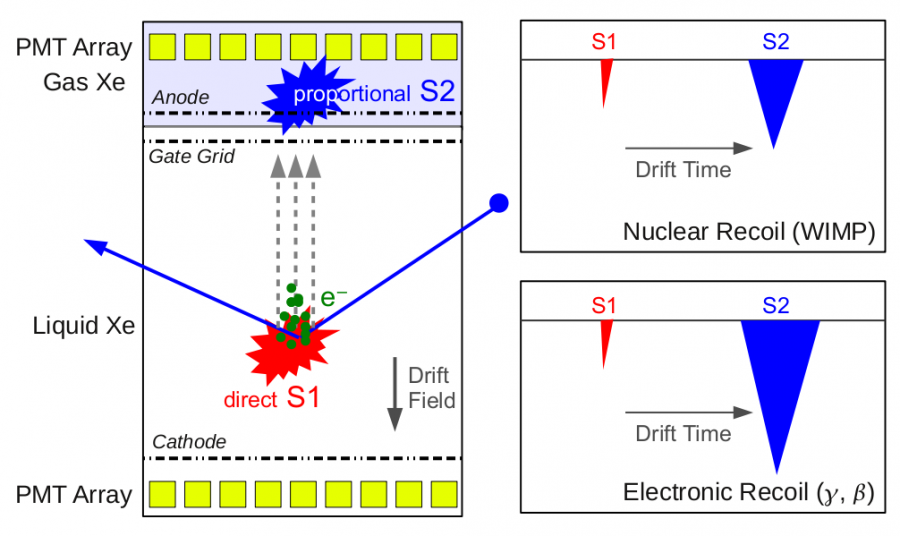
\includegraphics[width=0.95\textwidth]{figs/xe100TPC.png}
	\mycaption[TPC detection principle]{ Operational principle of the XENON TPC. The ratio S2/S1 provides separation between nuclear and electromagnetic recoils.}
	\label{fig:xe100TPC}
\end{figure}

The detector has been operating between the years 2008 and 2016, achieving an exclusion limit of $\sigma_{SI} = 1.1 \times 10^{-45}$ for a 50\,GeV WIMP~\cite{xe100_run_combination}. Additionally XENON100 excluded many interpretation trying to explain the tension with DAMA/LIBRE observation results. In Chapter~\ref{chap:EFT} I present an analysis done on the XENON100 data considering the EFT approach for high energy recoils~\cite{Aprile:2017aas}.  

\subsection{XENON1T}
\label{sec:xe1T}

The third phase of the XENON program is the XENON1T detector~\cite{Aprile:2017aty}. This detector is the first ton scale dual phase TPC  DM detector. It has been fully operating since 2016. The XENON1T TPC contains $~sim 3$\,tons of LXe (1\,ton in the FV) and has achieved the lowest background rate in DM detectors. This level of background is achieved by carefully selecting low radioactive materials, and by deploying the TPC in the middle of a 10 meters hight, 10 meters diameter water tank, which acts as an active cosmic muon veto and as a passive neutron shield. A view of XENON1T is shown in Fig~\ref{fig:xe1tLim}.

\begin{figure}[]
	\centering
	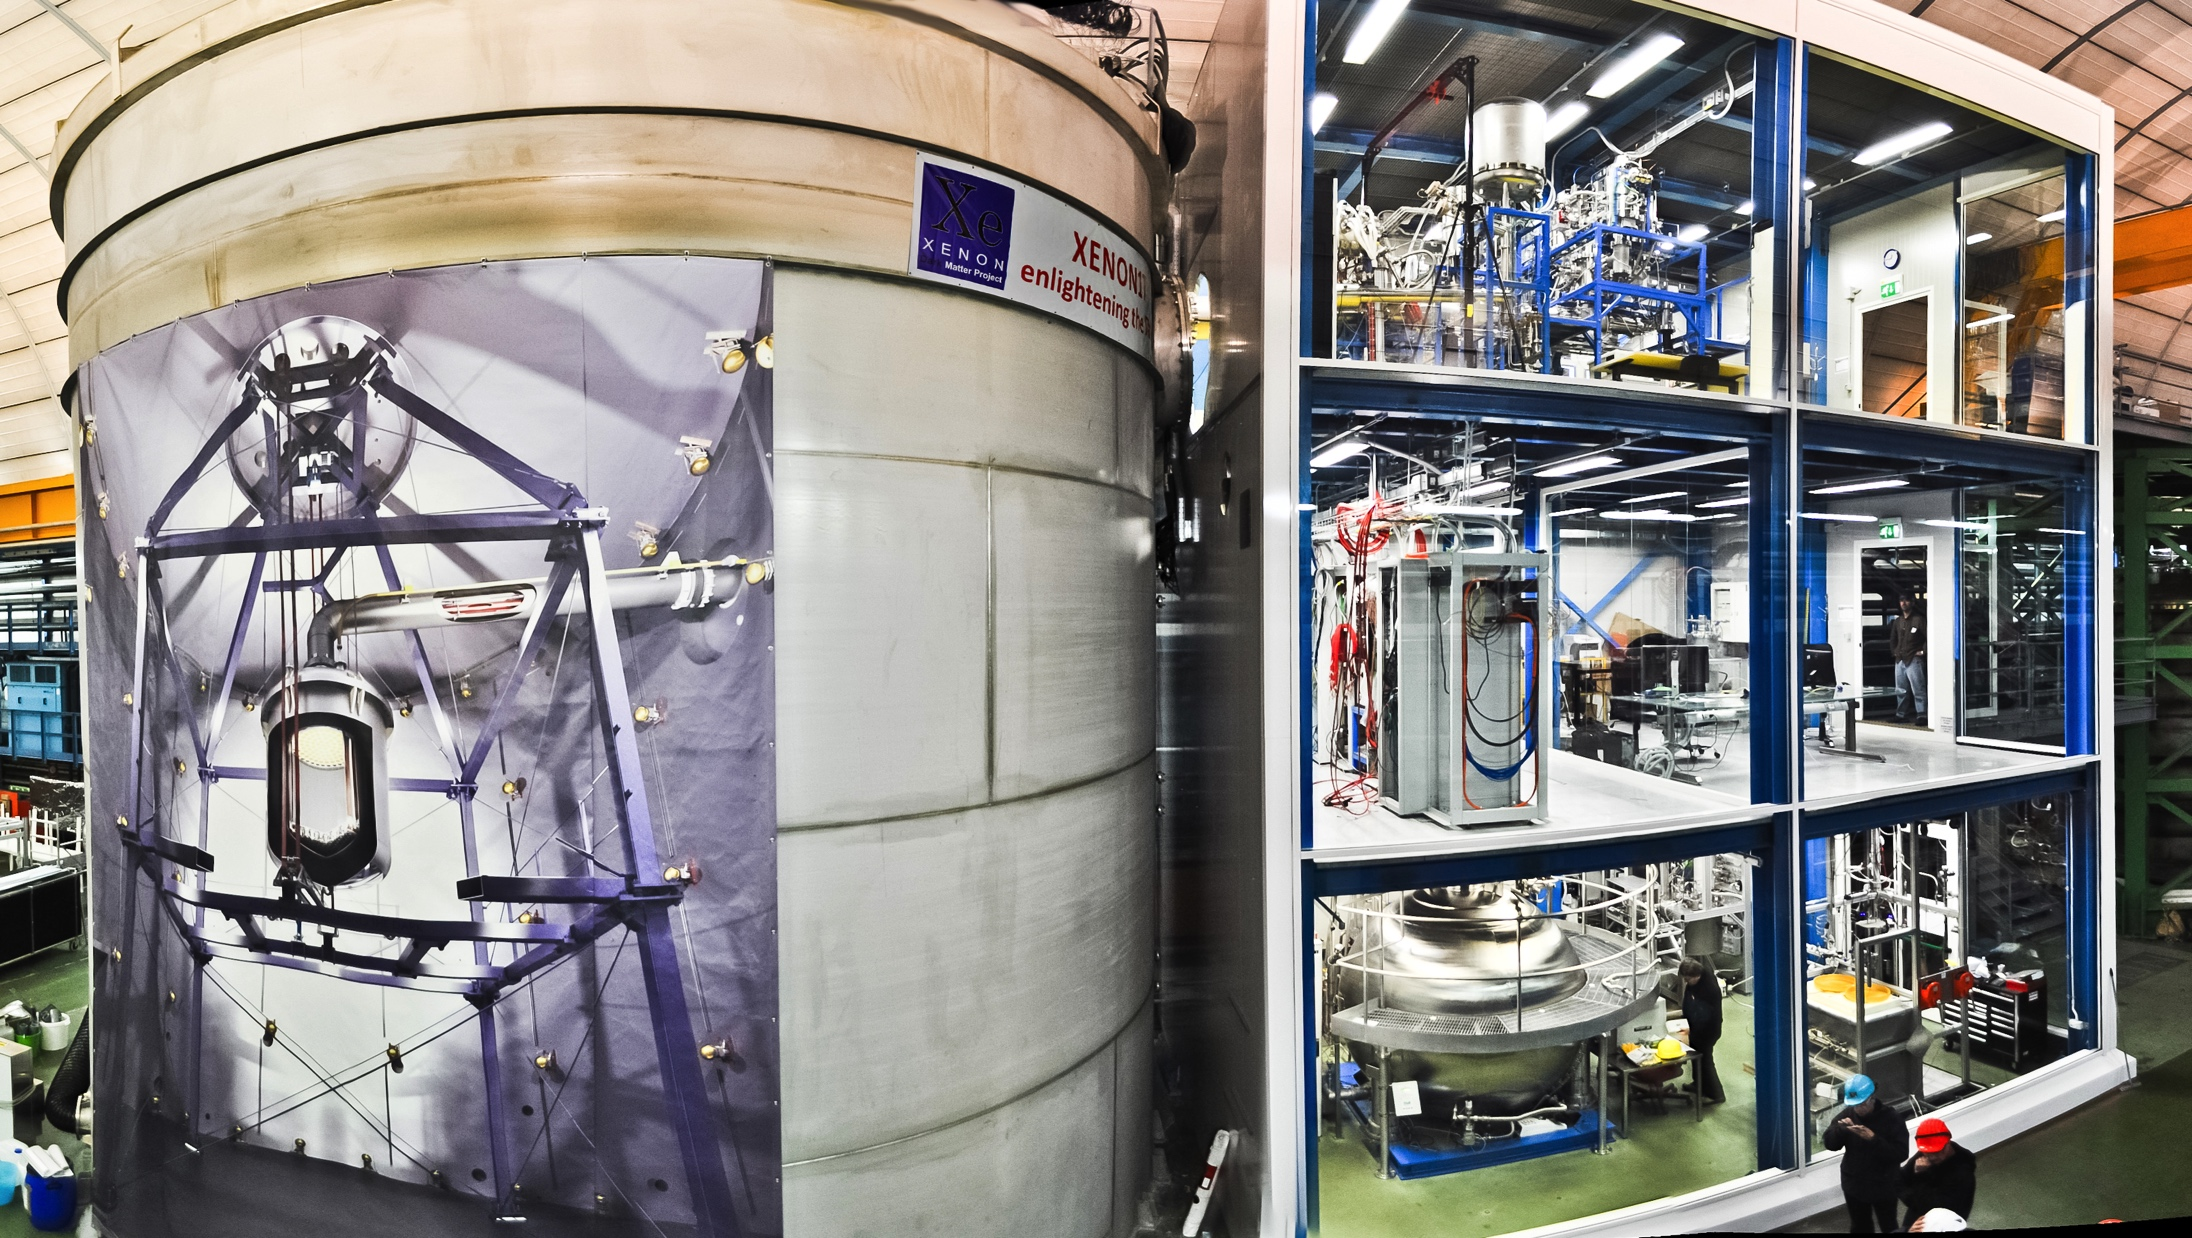
\includegraphics[width=0.95\textwidth]{figs/xe1tImg.png}
	\mycaption[XENON1T Image]{A picture of the XENON1T detector(left) and its control room (right)}
	\label{fig:xe1tLim}
\end{figure}

The first science run had an exposure of 1 month, achieving the most stringent  exclusion limit to date with a minimum of $7.7\times10^{-47}$\,cm$^2$ for a 35\,GeV WIMP, the full limit is shown in Fig.~\ref{fig:xe1tLim}. In Chap.~\ref{chap:calibration}, is a description of the calibration system of XENON1T.
 
\begin{figure}[]
	\centering
	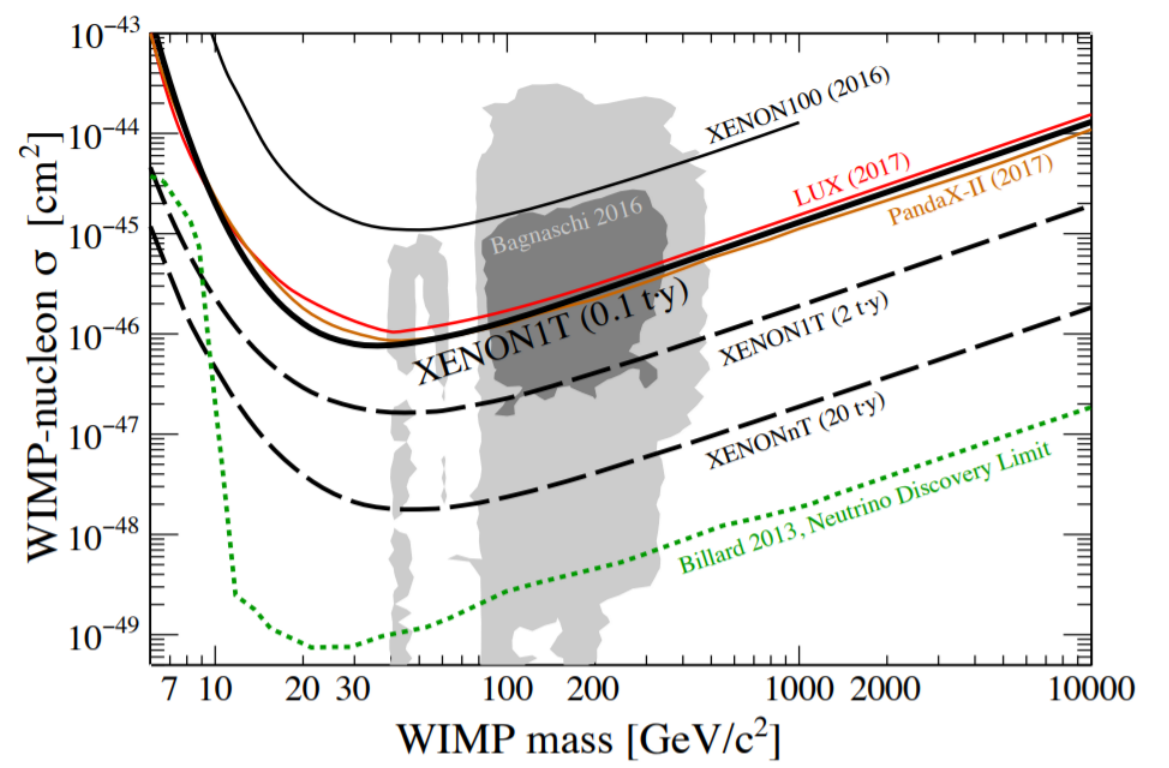
\includegraphics[width=0.95\textwidth]{figs/xe1tLimit.png}
	\mycaption[XENON1T exclusion limit]{The spin-independent WIMP-nucleon cross section limits as a function of WIMP mass at 90\% confidence
level.}
	\label{fig:xe1tLim}
\end{figure}


\subsection{XENONnT}
\label{sec:xenT}

The fourth and final phase of the XENON program is the XENONnT detector. Unlike other phases, this phase will be integrated inside the infrastructure of its ancestor XENON1T. The main upgrade will be the replacement of the inner vessel of XENON1T to a larger vessel which contains roughly $\sim8$\,ton of LXe. The projected sensitivity of XENONnT is estimated to be $1.6\times10^{-48}$\,cm$^{2}$ 
%\subsection{Subsection}
%\label{subsec:subsec01}
%
%Begins a subsection.
%
%%A figures matrix.
%\begin{figure}[t!]
%\centering
%\begin{minipage}{3.3cm}
%    \centering
%    \subtop[]{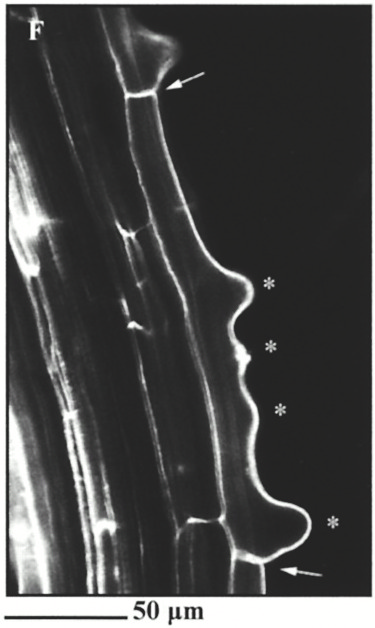
\includegraphics[height=0.28\textheight]{fig01/Nswellings}\label{sf:multiRH02a}}
%\end{minipage}
%\hspace{0.5cm}
%\begin{minipage}{3.3cm}
%    \centering
%    \subtop[]{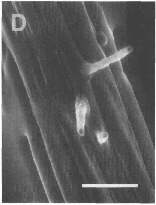
\includegraphics[height=0.27\textheight]{fig01/Mswellings}\label{sf:multiRH02b}}
%\end{minipage}
%\hspace{1.3cm}
%\begin{minipage}{3.3cm}
%    \centering
%    \subtop[]{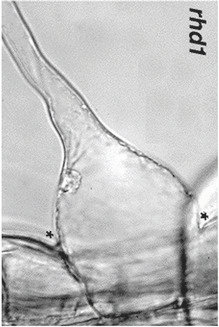
\includegraphics[height=0.27\textheight]{fig01/rhd1}\label{sf:multiRH02c}}
%\end{minipage}
%%\\ \vspace{0.1cm}
%%\begin{minipage}{10cm}
%    \centering
%    \subtop[]{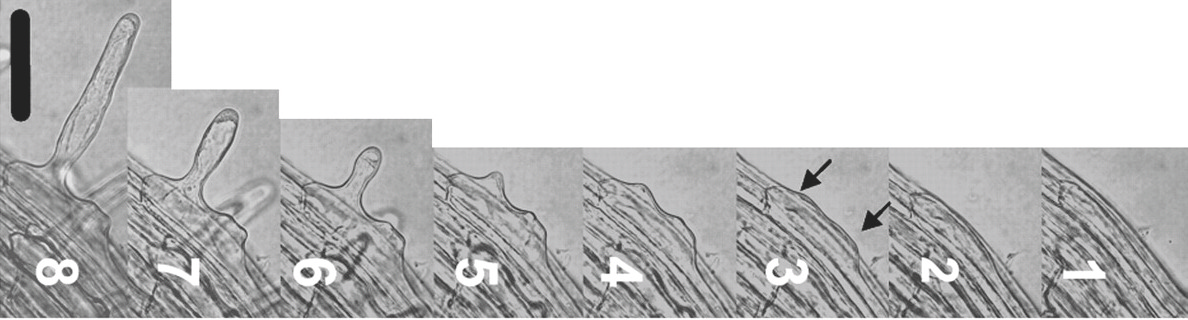
\includegraphics[height=0.145\textheight]{fig01/mutantrhd6}\label{sf:multiRH02d}}
%\end{minipage}
%\\ \vspace{0.1cm}
%\begin{minipage}{10cm}
%    \centering
%    \subtop[]{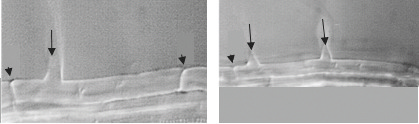
\includegraphics[height=0.16\textheight]{fig01/auxab}\label{sf:multiRH02e}}
%\end{minipage}
%\mycaption[Hair-forming mutant cells.]{(a) A mutant RH cell. Asterisks show multiple sites of RH initiation in a single root hair cell (indicated by the arrows). Figure reproduced from \cite{rigas01}. (b)~Hair-forming cell with three RH initiation locations. The bar represents $50\mu m$. Figure reproduced from \cite{massuci01}. (c) Large bump in mutant {\itshape rhd1}. Figure reproduced from \cite{griersonRH}. (d) Mutant overexpressing gene {\itshape ROP2}; from right-hand to left-hand, numbers indicate progressive snapshots at different times. RH initiation sites are indicated by the arrows. The bar represents $75\mu m$. Figure reproduced from~\cite{mjones01}. (e)~Mutants affected by auxin. On the left-hand side, RH site is farther away from the apical end (left arrow cap); on the right-hand side, multiple RH locations (arrows). Figure reproduced from~\cite{payne01}.}
%\label{fig:multiRH02}
%\end{figure}
%
%% A single figure
%\begin{figure}[t!]
%	\centering
%	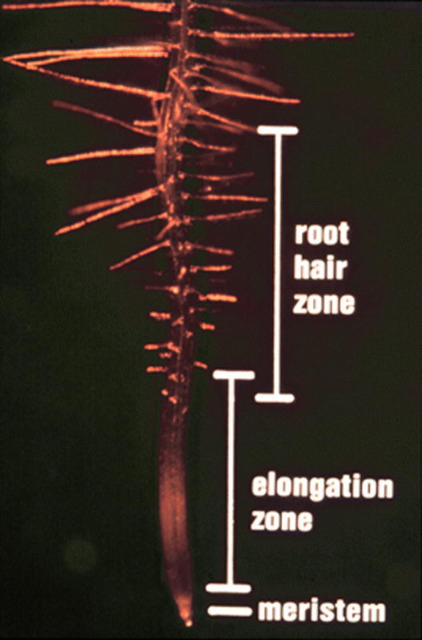
\includegraphics[height=0.35\textheight]{fig01/devepzones}
%	\mycaption[Developmental zones of an Arabidopsis root.]{Developmental zones of an Arabidopsis root. Figure reproduced from \cite{griersonRH}.}
%	\label{fig:RHP02}
%\end{figure}

%=========================================================